\documentclass[a4paper]{article}

\usepackage{geometry}
\usepackage{indentfirst}
\usepackage{verbatim}
\usepackage{amsmath,amssymb}
\usepackage{amsthm}
\DeclareMathOperator*{\argmax}{arg\,max}
\usepackage{amsthm}
\usepackage{bm}
\usepackage{bbm}
\usepackage{graphicx}
\usepackage{float}
\usepackage{color}
\usepackage{algorithm}
\usepackage{algorithmic}
%\renewcommand{\algorithmicrequire}{\textbf{Initialization:}}
%\renewcommand{\algorithmicensure}{\textbf{Inference:}}

\geometry{left=3cm,right=3cm,top=3.75cm,bottom=3.75cm}
\setlength{\parindent}{0em}
\setlength{\parskip}{1em}


\begin{document}

\newtheorem{thm}{Theorem}
\newtheorem*{thm*}{Theorem}
\newtheorem{lem}{Lemma}
\newtheorem{cla}{Claim}
\newtheorem{prop}{Proposition}

\title{Final report}

\author{Lei Zhong, Hantian Zhang, Jian Zhang}
\date{}
\maketitle

\abstract{We did more experiment with different parameters during the Milestone 4. We optimized the code and visualized the results as a video on youtube\cite{youtube}. In this final report, we will summarize over the whole three-month project, demonstrate the results and point out some future work}

\section{Introduction}
Climate change is an issue of ever increasing significance to both policy makers and the public, especially as the impact of climate change on global and local economies has become clear. People care about this critical issue, and this interest is reflected in news headlines and across global social media.

Geologists and climatologists have developed many traditional methods the get more insight of this problem. They look into evidences from temperature measurements and proxies, historical and archaeological evidence, glaciers, arctic sea ice loss, vegetation, precipitation, sea level change and so on. They have also built many satellites and monitoring stations that are collecting large volumes of data everyday to help with the analysis. However, these traditional methods are mostly based on hypothesis testing methods and can't make full use of these automatically collected data, as the data volume is too big to handle. It is natural that novel methods that are able to deal with big data can play an important role in the climate change research.

We developed a system to cluster and visualize the GHCN-D data\cite{GHCN-D}.
GHCN-D is a dataset that contains daily weather observations over global land areas.
Like its monthly counterpart, GHCN-Daily is a composite of climate records from
numerous sources that were merged together and subjected to a common suite of quality assurance reviews. The archive includes the following meteorological elements: daily maximum temperature, daily minimum temperature, temperature at the time of observation, precipitation (i.e., rain, melted snow), snowfall, snow depth, other elements where available. The data we used dates from 1763 to 2014 and has approximately 100 Gigabytes total volume.


%Why is this problem interesting or useful?
%Why do we need a new system?
%Which alternative/traditional techniques can be used to solve the problem

%What is the main new contribution of your approach
%How does your solution compare to existing work



\section{The System Architecture}

\subsection{Description of the Architecture and Tools used}
As is shown in Figure \ref{fig:archi}, CLUE has four main steps : Feature Extraction, Sampling, Clustering and Visualization. The tools we use includes Amazon Elastic MapReduce\cite{EMR}, Scikit-learn\cite{sklearn} library and Google Map API\cite{GoogleMap}. The four steps are illustrated in details in the followling part.
\begin{figure}[htbp]
				\centering
				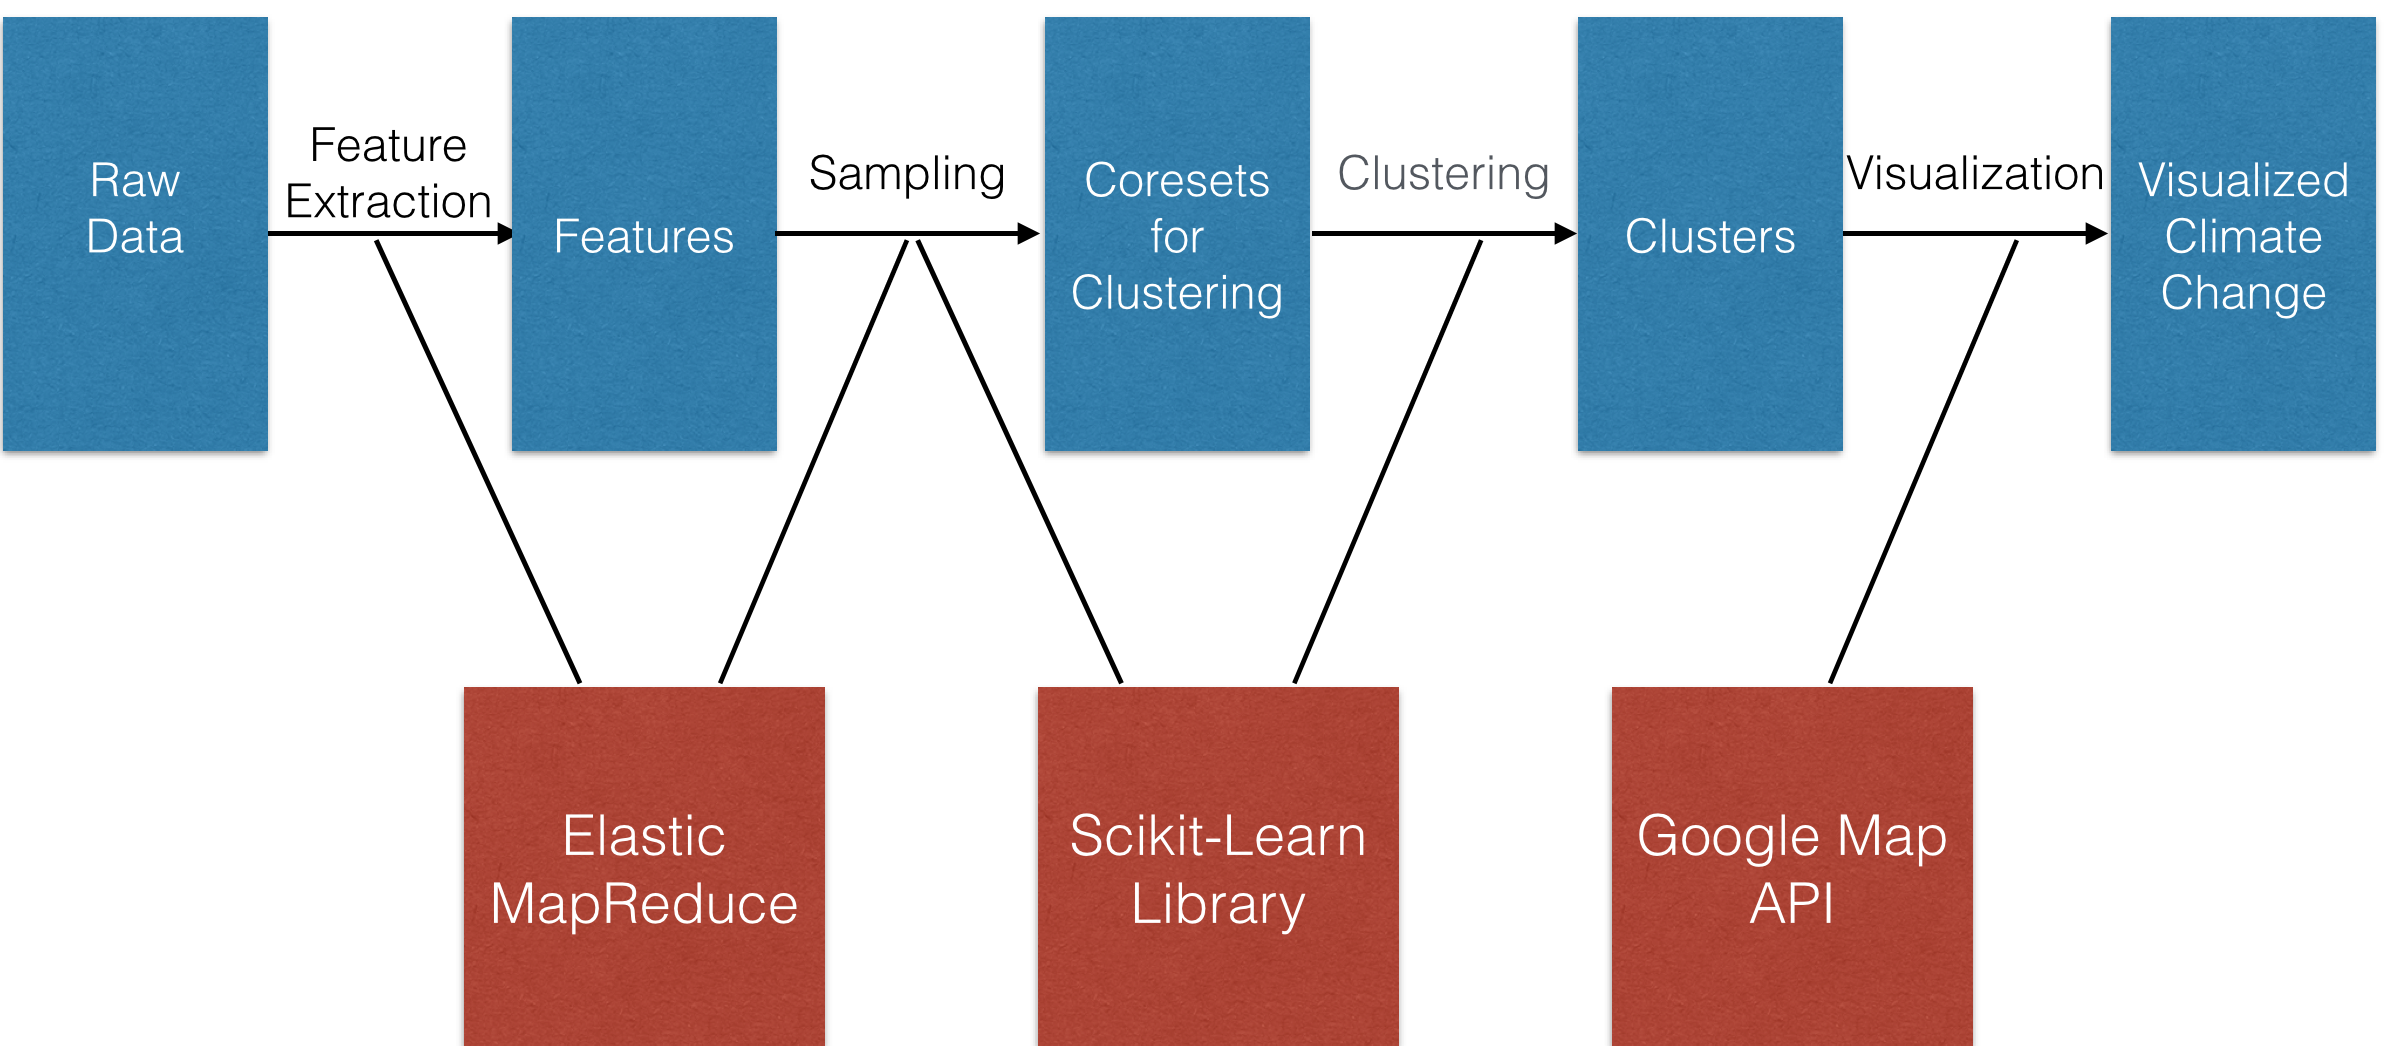
\includegraphics[width=0.9\textwidth]{images/Architecture.png}
				\caption{Architecture of CLUE}
				\label{fig:archi}
 \end{figure}
 
\subsubsection{Feature Extraction}
The raw data includes the climate data from 1763 to 2014, the total volume of raw data is about 100 Gigabytes, which is too big to fit in the memory. So we use Amazon Elastic MapReduce to calculate features. We use the same features setting with the previous milestone. The feature extraction consists of 3 sub-steps, including calculating features for existing data, filling in the missing value using the mean value of the feature value of all other existing data and normalizing data. Each of these sub-steps is done by a map-reduce task because of the huge volume of data. Through feature extraction, we get about 300 million 60-dimentional data points.

\subsubsection{Sampling}
We want to use all data points to run clustering. However, we use the k-means function in the scikit-learn library to compute clusters. It is impossible for that k-means function to run on 300 million of data points. We have two choices of handling this. One is to write a parallel k-means function that can run on Amazon EMR, the other one is to sample these data points so that the sample points are able to represent all the data points with the minimum loss of information. We choose the second approach and use coreset for k-means clustering. The coreset is a set of data points that is used to run the weighted k-means clustering. Each point in the coreset represents some original data points that are near to it. These data points are assigned the same label as the point in the coreset. The coreset sampling is done by an iterative step, where in each step, we uniformly sample some data points, calculate distance to the nearest point in the sampling set for every data point, remove data points whose distance to the nearest point in the sampling set are below median. Iterate this step until the number of remained data points is smaller than a pre-defined number and we get a coreset sampling of data. In addition to coreset sampling, we could also run the clustering on the whole data for a couple of years for detailed information in these years, which is done in milestone 2.


\subsubsection{Clustering}
Having the coreset whose size is reasonable, we can run weighted k-means algorithm on the coreset and calculated all the centroids. The last step is to assign each data point to the nearest centroid and give that data a label. This step is also done by a map-reduce task.

\subsubsection{Visualization}
For the visualization part, we used the same technique that we have used in milestone 2. We used Google Map API to visualize the clustering result. For each year, all the stations in that year are placed on the map according to its location and the stations in the same cluster have the same color. We did an animation to show the change of clusters that reflects climate change.

\subsection{Limits in Scalability and Possible Improvements}
We have used most data that is available, however, due to the sampling process, the pattern of the result of clustering is not as obvious as the previous milestone. The main limit is the scalability of the clustering algorithm. I think coreset sampling is a good way to handle this, but due to the time limit, the coreset sampling we implemented has a lot of room for improvement and the clustering result is not as good as imagined. We would like to improve our sampling method and try different parameters for better sampling and clustering result. Also, we would like to write a parrallel k-means algorithm so that we can use more data points if possible.

\paragraph{to add}
In addition to coreset sampling, we could also run on the whole feature, 

\section{Performance Measurements and Results}

\subsection{Performance metrics}
There are three common performance metrics, we have our own way to measure:
\begin{itemize}
    \item Execution time: one is run-time, the other is normalized instance hour;
    \item Memory-consumption \& number of machines: peak memory of mapper and reducer, see Table \ref{table:m3}. We use m3.2xlarge and one master, two cores.
    \item Solution quality: our project is quite innovative and there is no existing work. We can only compare our results with differnt parameters by topographical world map\cite{world}.
\end{itemize}

\begin{table}[htbp]
    \centering
    \label{table:m3}
    \begin{tabular}{|l|l|l|l|}
        \hline
        Model & vCPU & Mem (GiB) & SSD Storage (GB) \\
        \hline
        m3.medium & 1 & 3.75 & 1 x 4  \\
        m3.large  & 2 & 7.5 & 1 x 32 \\
        m3.xlarge & 4 & 15 & 2 x 40 \\
        m3.2xlarge& 8 & 30 & 2 x 80 \\
        \hline
    \end{tabular}
    \caption{Instance types}
\end{table}

\subsection{Result of recent four decades}
Same as Milestone $3$, we selected the year $1983$, $1993$, $2003$ and $2013$ to show the results. The size of raw compressed dataset is as showing in the Table \ref{table:4year}.

\begin{table}[htbp]
    \centering
    \label{table:4year}
    \begin{tabular}{|l|l|l|l|l|}
        \hline
        Year & 1983 & 1993 & 2003 & 2013 \\
        \hline
        Compressed Size & 155MB & 152MB & 159MB & 166MB \\
        \hline
        Original & 912.4MB & 899.7MB & 960.7MB & 987.2MB \\
        \hline
    \end{tabular}
    \caption{Size of dataset in selected years}
\end{table}

We kept adjusting the parameters until we found the result is resonable. The following pictures are snapshots from $150$ clusters, $500$ iterations. From the pictures we can see that there do exist some pattern in the same region in different years. But generally, the shape of clusters would note be the same.

\begin{figure}[htbp]
    \centering
    \begin{tabular}{c}
        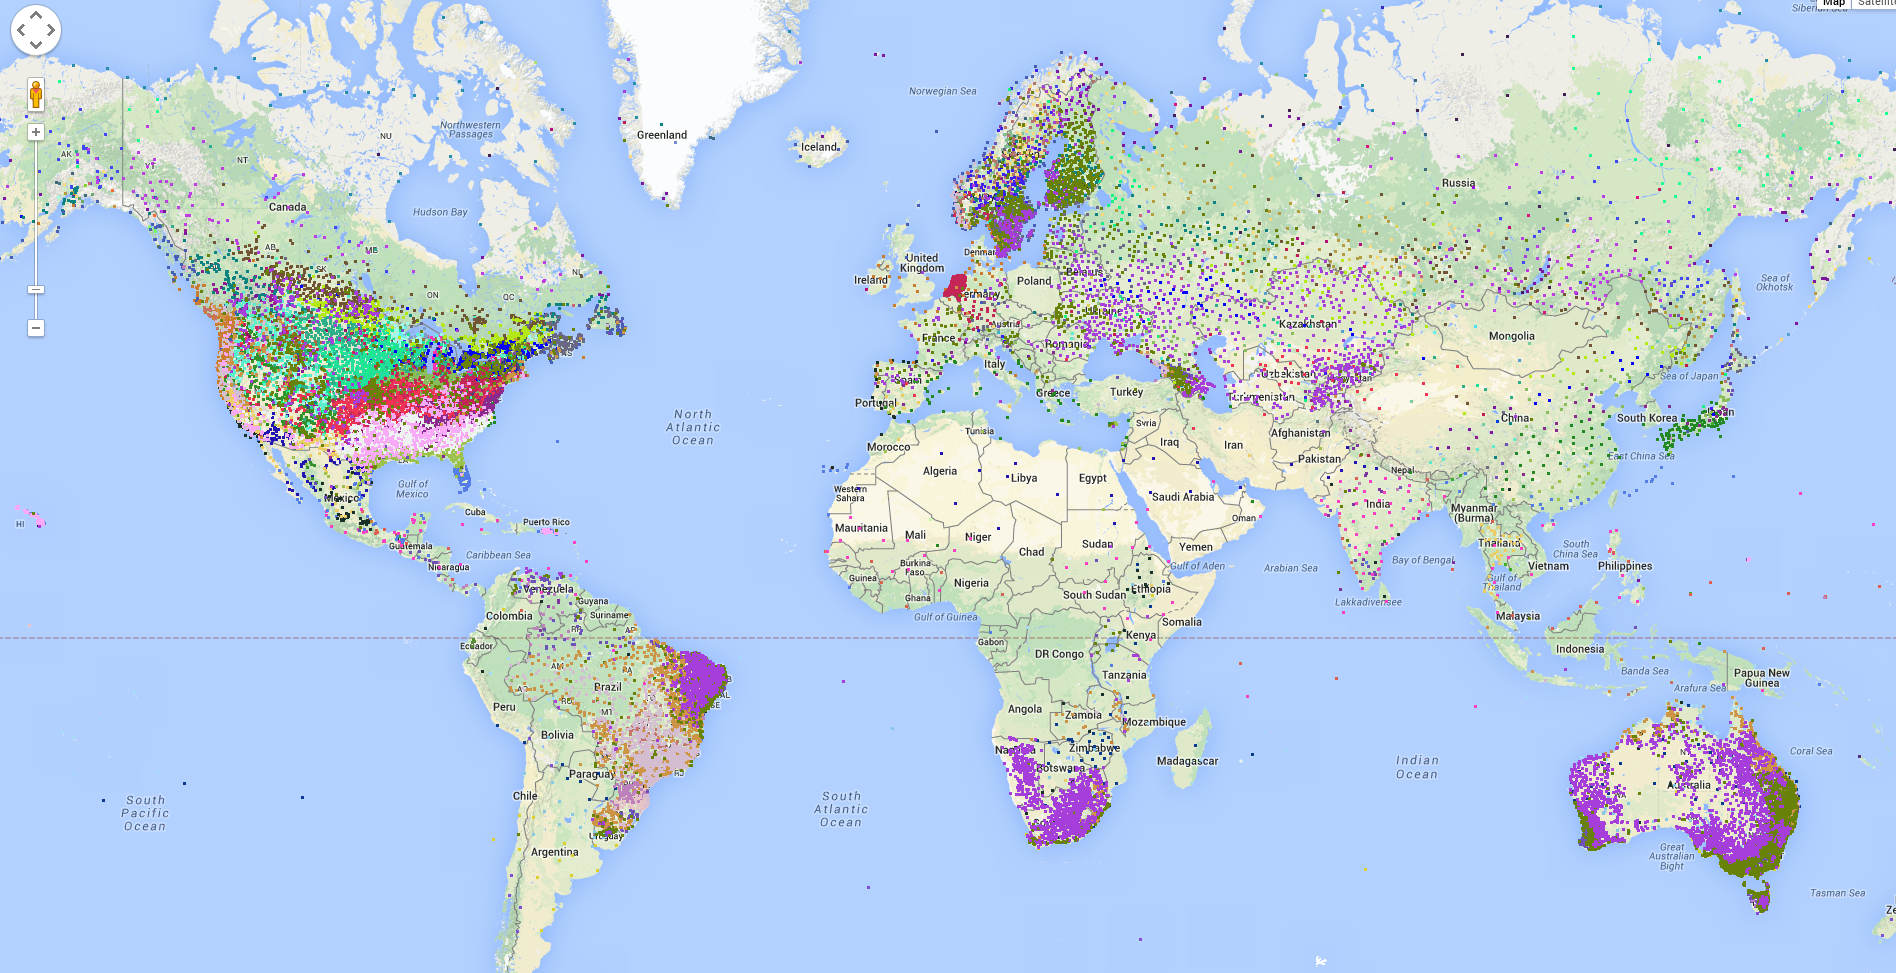
\includegraphics[width =\linewidth]{images/1983.png}\\1983\\
        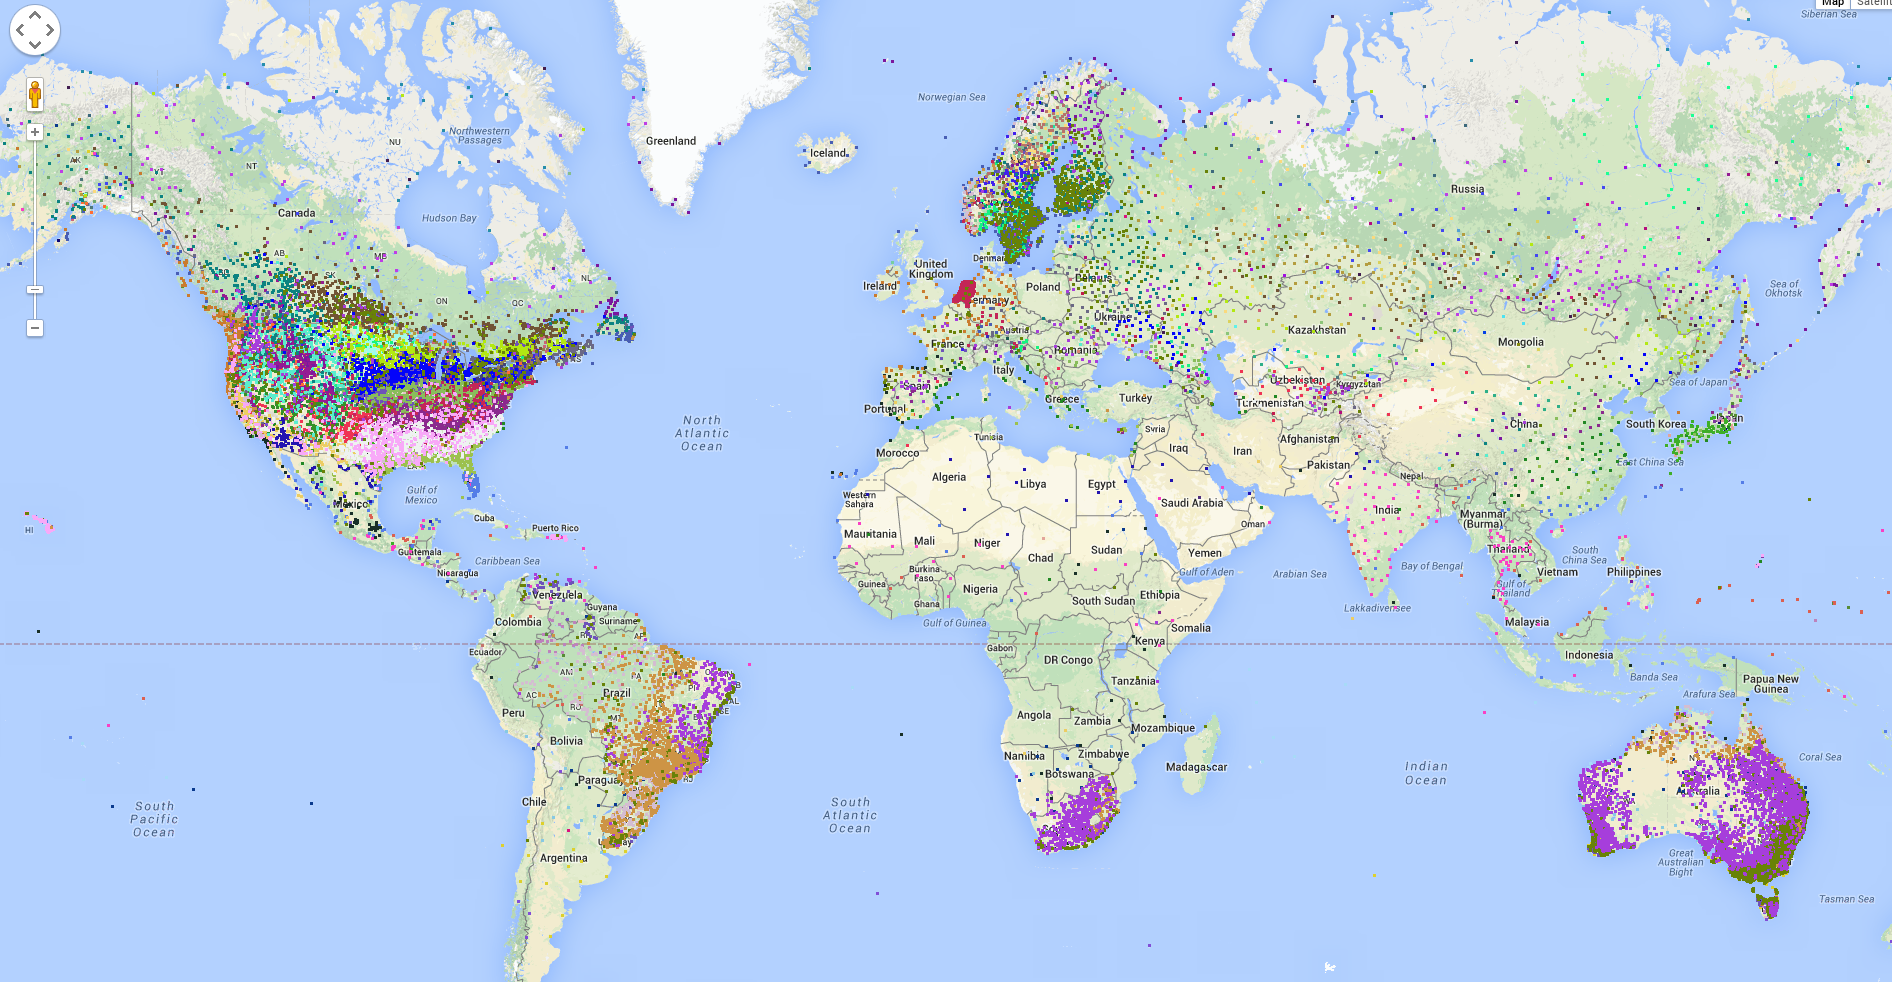
\includegraphics[width =\linewidth]{images/1993.png}\\1993\\
    \end{tabular}
    \caption{Clustering results of 1983 and 1993.}
\end{figure}

\begin{figure}[htbp]
    \begin{tabular}{c}
        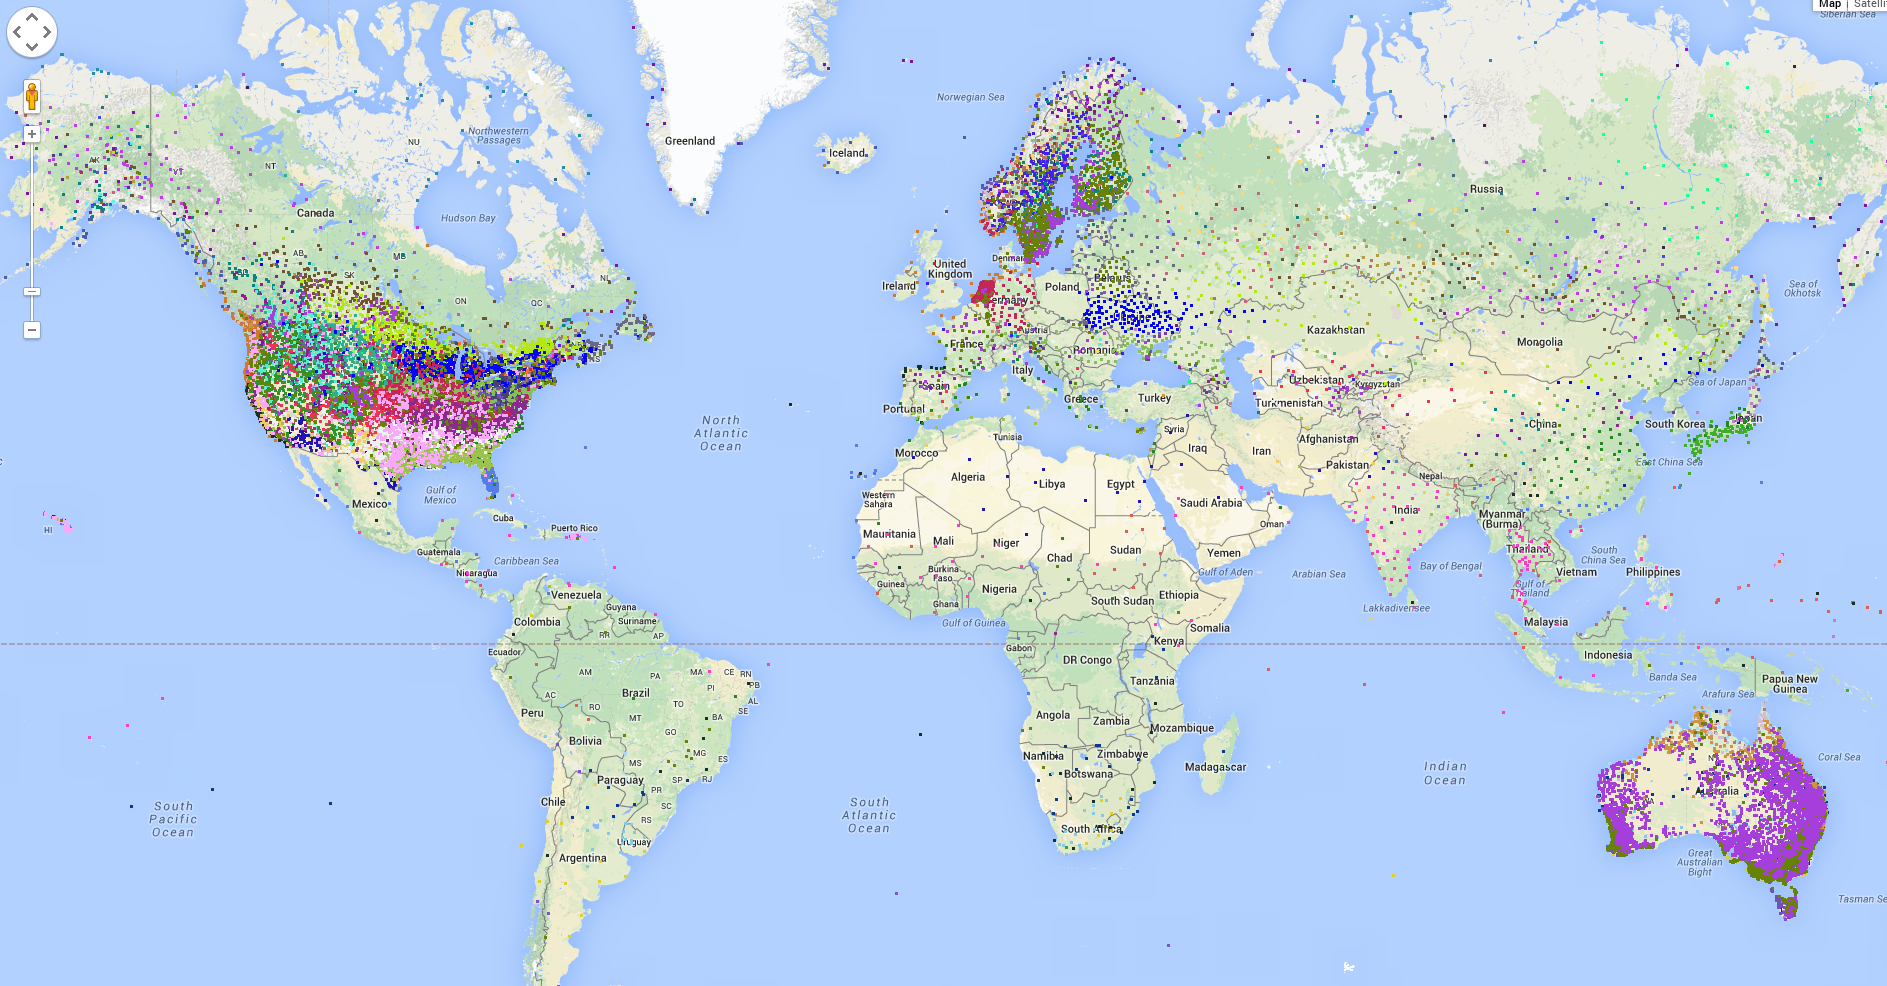
\includegraphics[width =\linewidth]{images/2003.png}\\2003\\
        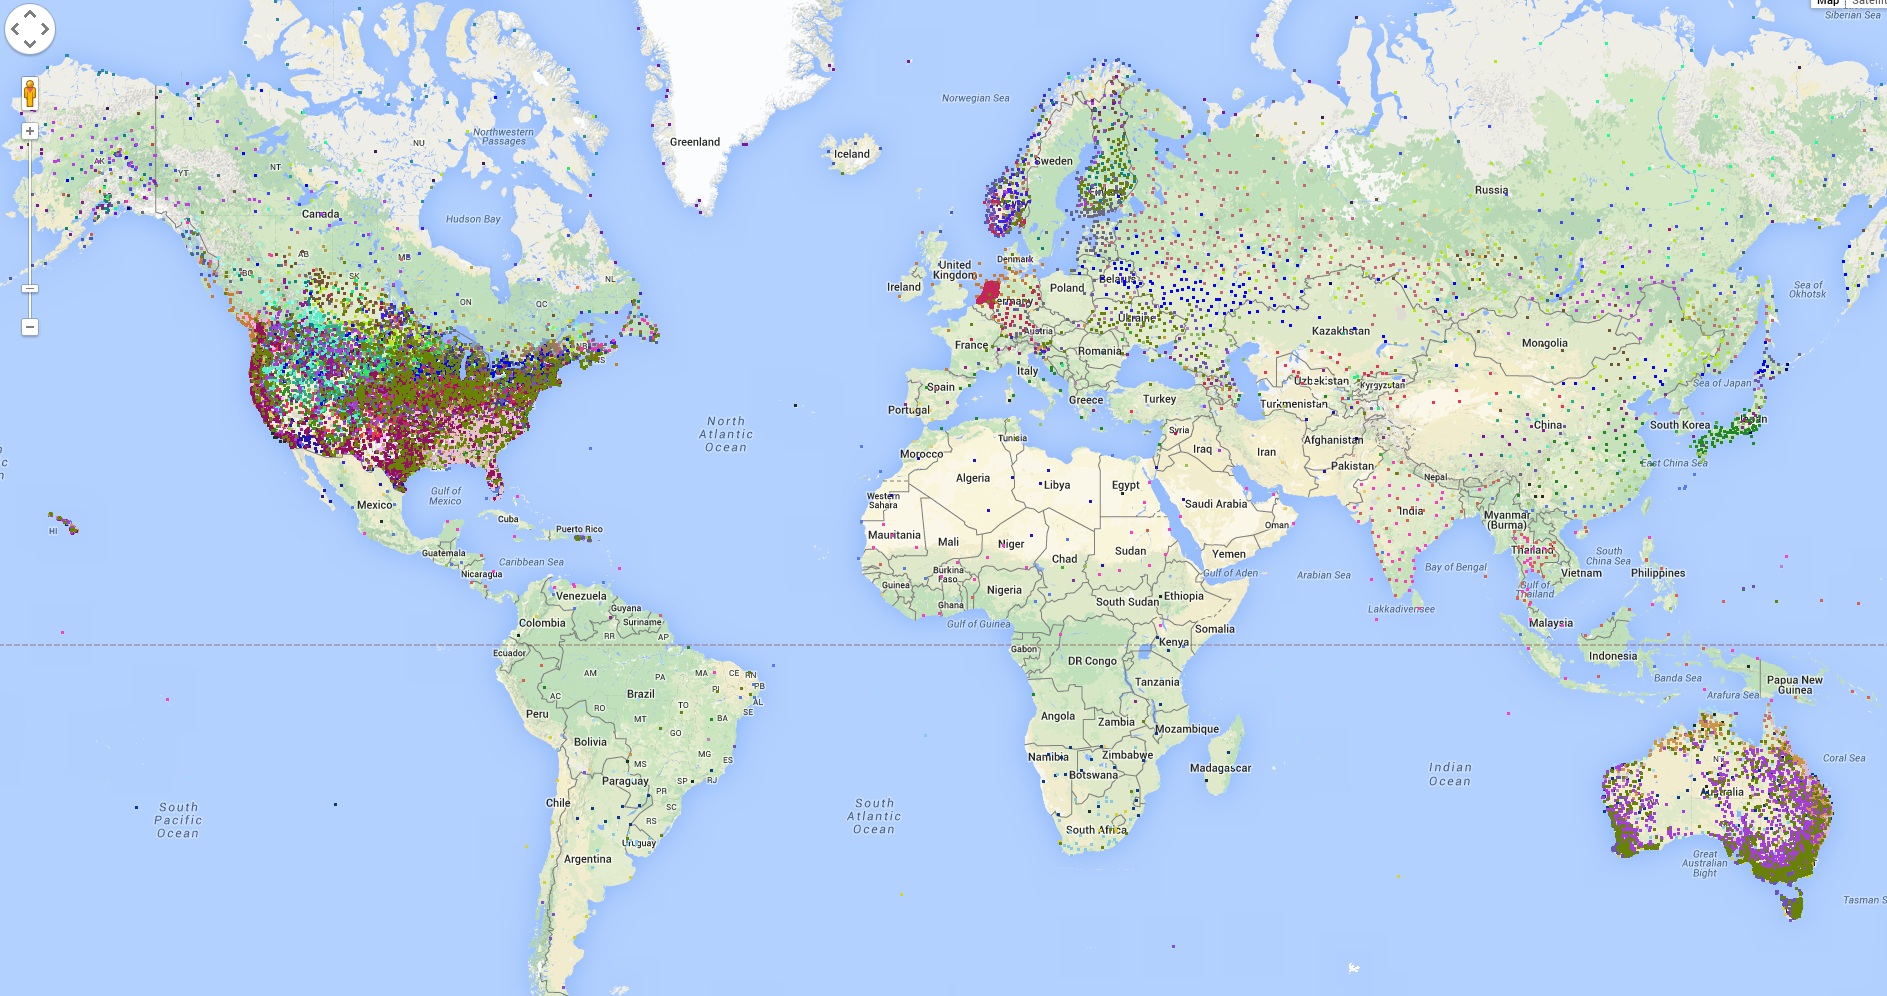
\includegraphics[width =\linewidth]{images/2013.png}\\2013\\
    \end{tabular}
    \caption{Clustering results of 2003 and 2013.}
\end{figure}

Compared with results in milestone $3$, there are two major improvements.
\begin{itemize}
    \item More clusters (which are different colors) are observed;
    \item Less mising points on the map;
\end{itemize}

\subsection{Result of more than a century}

At next step, we adjusted the parameter to less clusters. Because the former years have really small recorded weawther information, it's unnecessary to run many clusters. When we run with $90$ clusters, $500$ iterations to check if there is any similar pattern to the extent of a century. We have chosen the years $1876$, $1896$, $1904$, $1940$, and $2010$ with the size shown in Table \ref{table:5years}. The values are varying from $900K$ to $184M$\footnote{
The results before $1876$ is meaningless since there were not enough data.}.

\begin{table}[htbp]
    \centering
    \label{table:5years}
    \begin{tabular}{|l|l|l|l|l|l|}
        \hline
        Year & 1876 & 1896 & 1904 & 1940 & 2010 \\
        \hline
        Compressed & 900KB & 18MB & 32MB & 73MB & 184MB \\
        \hline
        Original & 5.5MB & 110.2MB & 201.7MB & 441.4MB & 1GB \\
        \hline
    \end{tabular}
    \caption{Size of dataset in selected years}
\end{table}

\begin{figure}[htbp]
    \centering
    \begin{tabular}{c}
        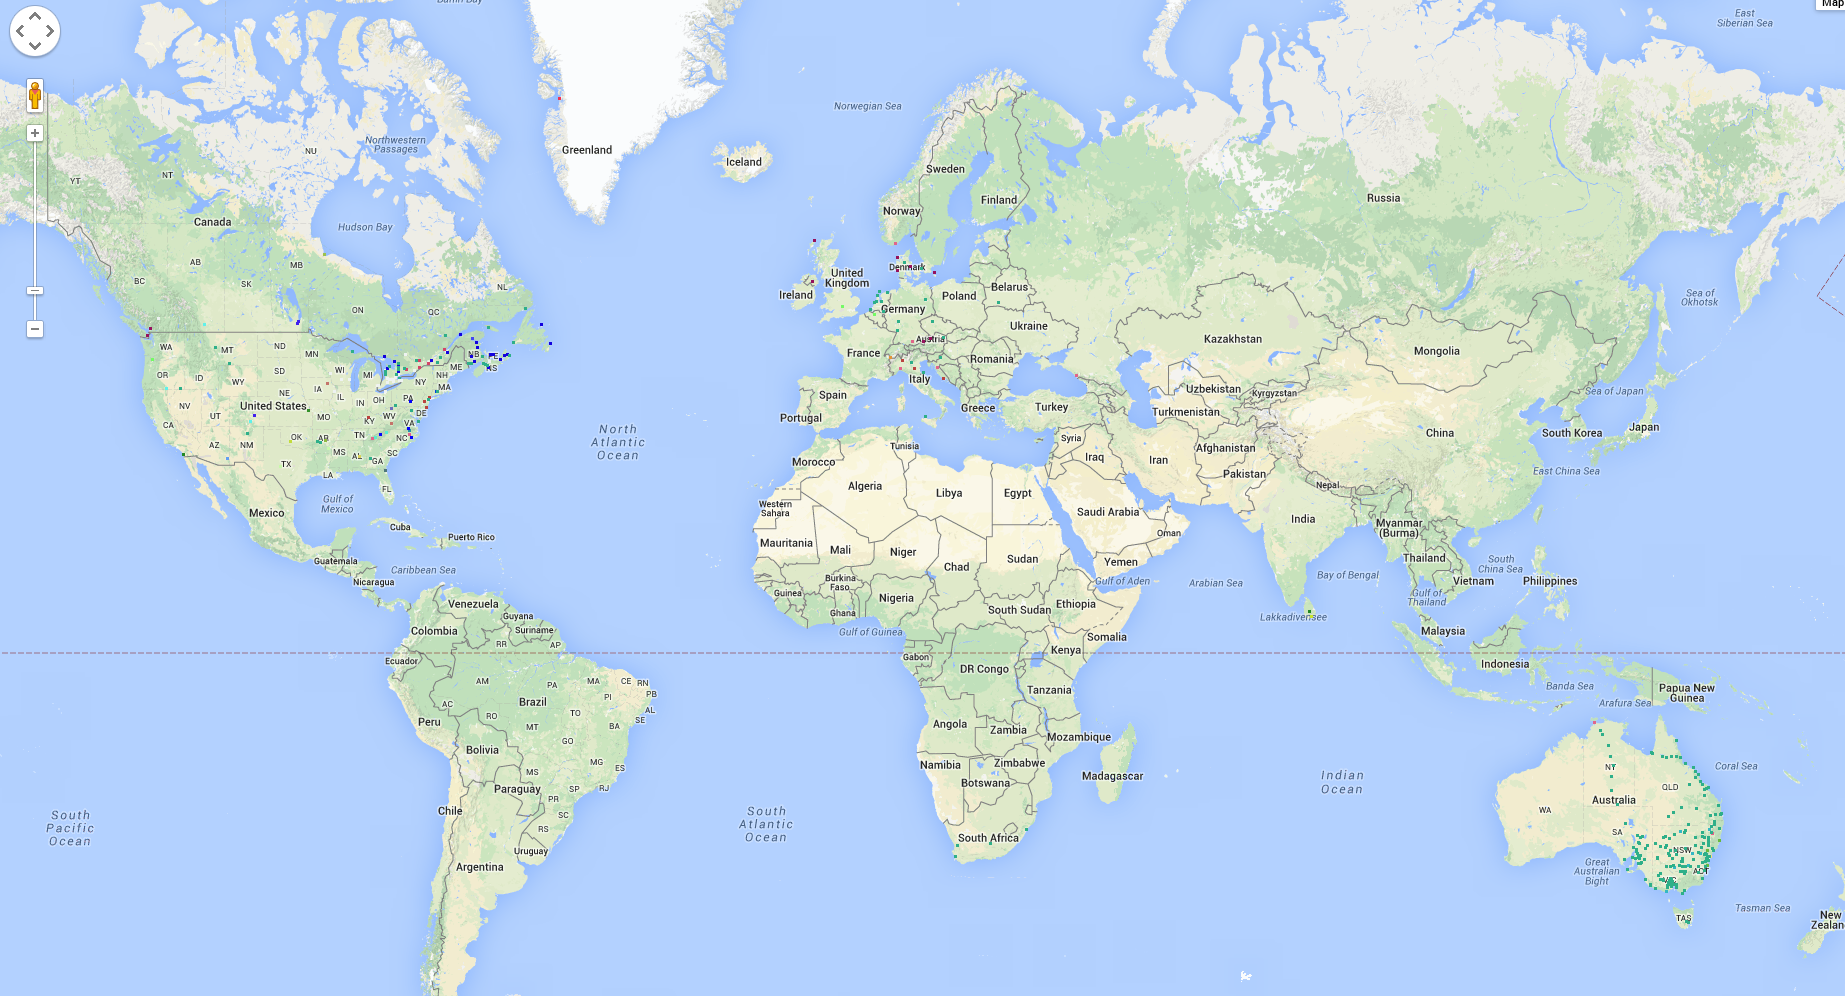
\includegraphics[width =\linewidth]{images/1876.png}\\ 1876\\
        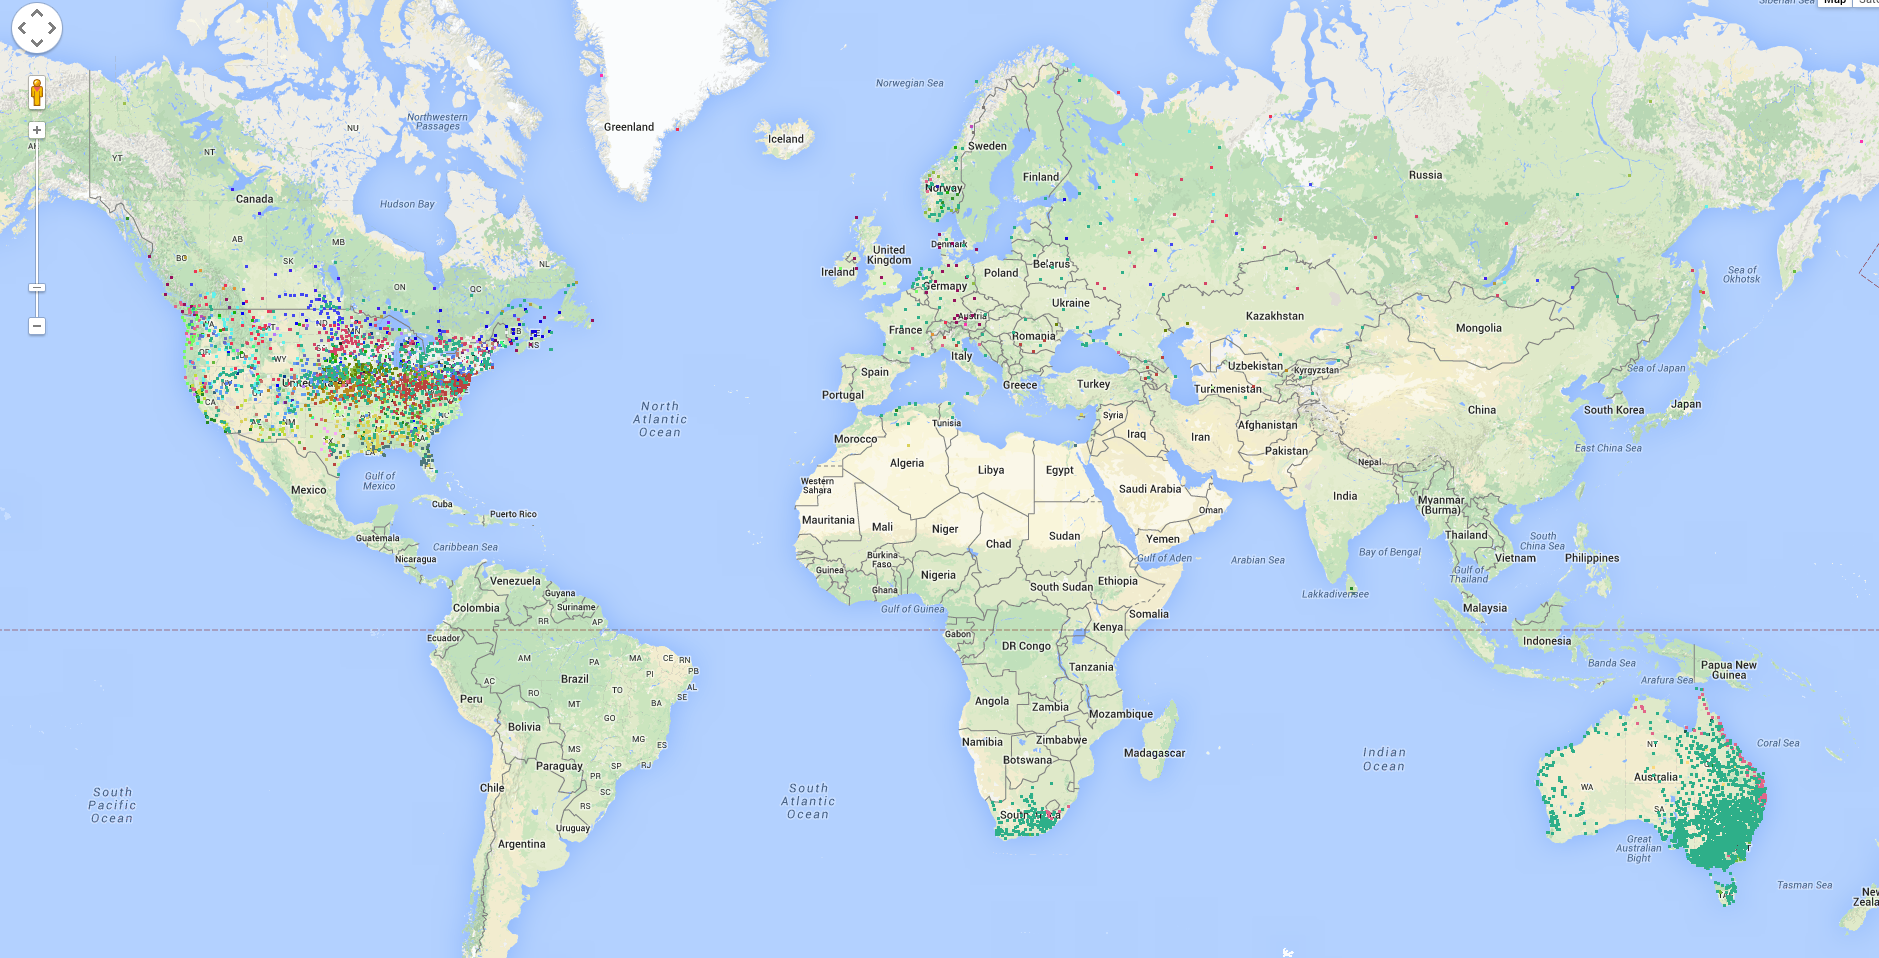
\includegraphics[width =\linewidth]{images/1896.png}\\ 1896\\
   \end{tabular}
    \caption{Clustering results of 1876 and 1896.}
\end{figure}

\begin{figure}[htbp]
    \centering
    \begin{tabular}{c}
        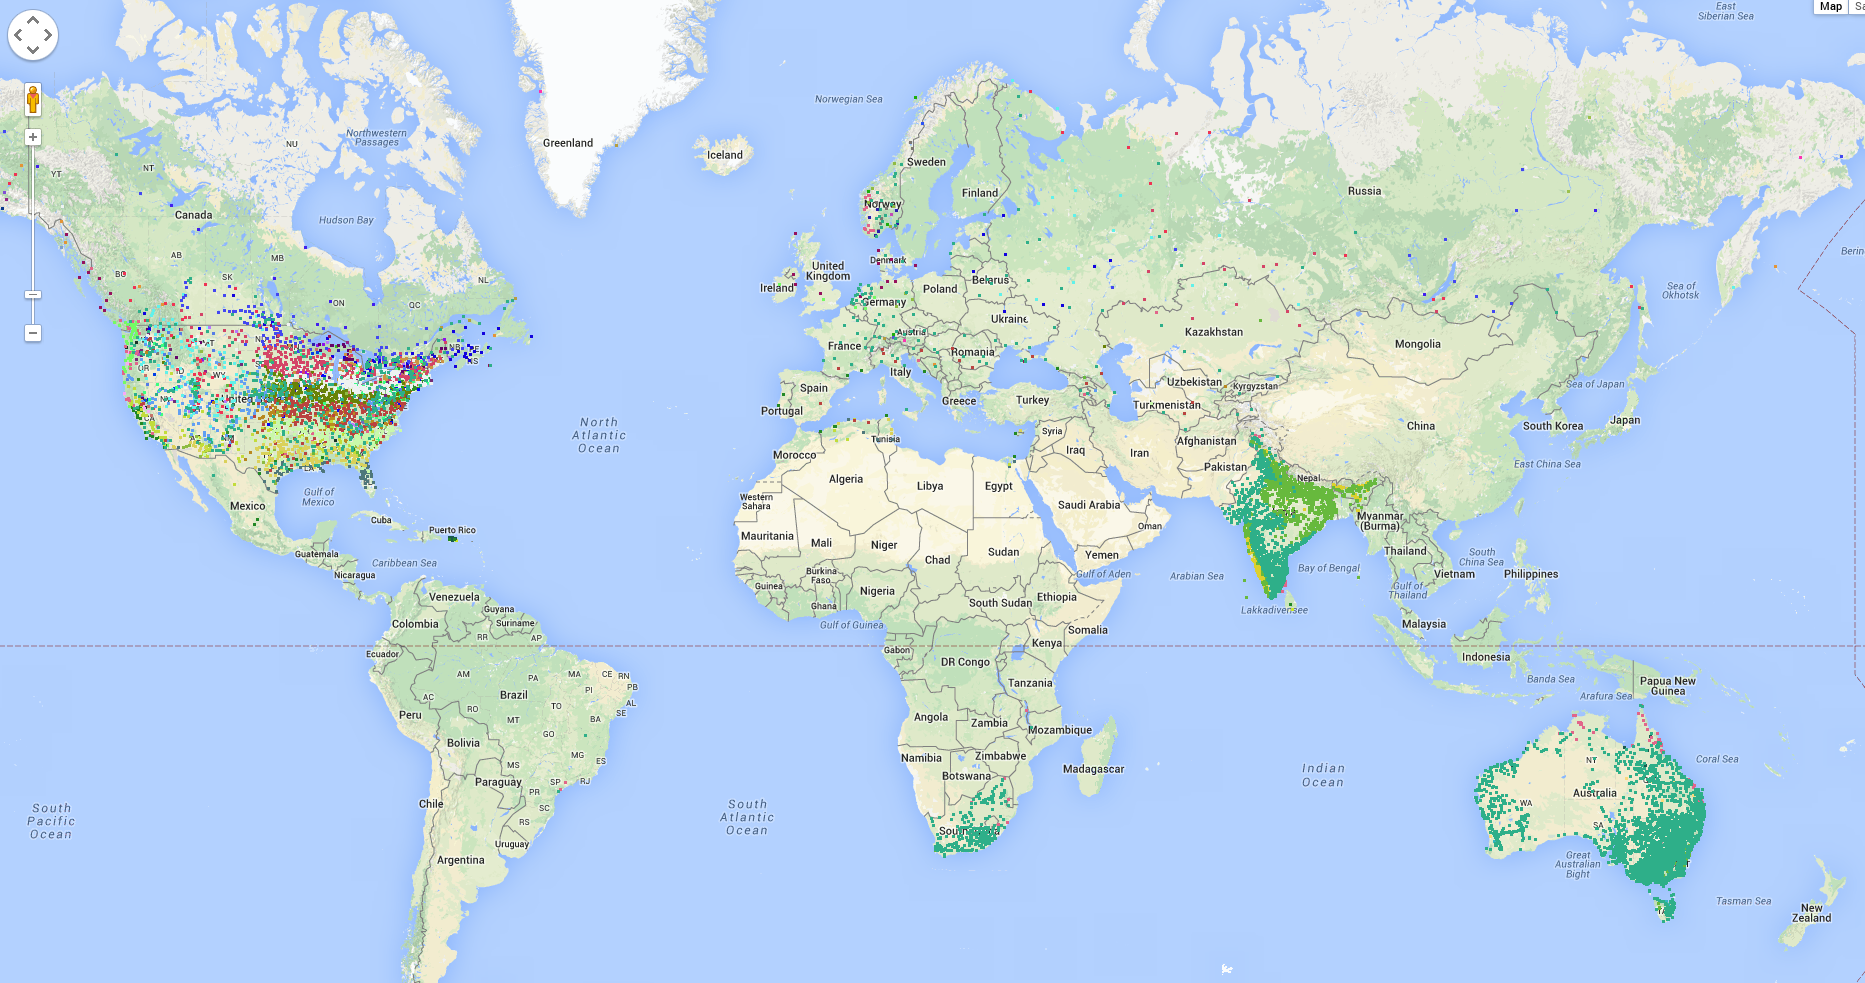
\includegraphics[width =0.8\linewidth]{images/1904.png}\\ 1904\\
        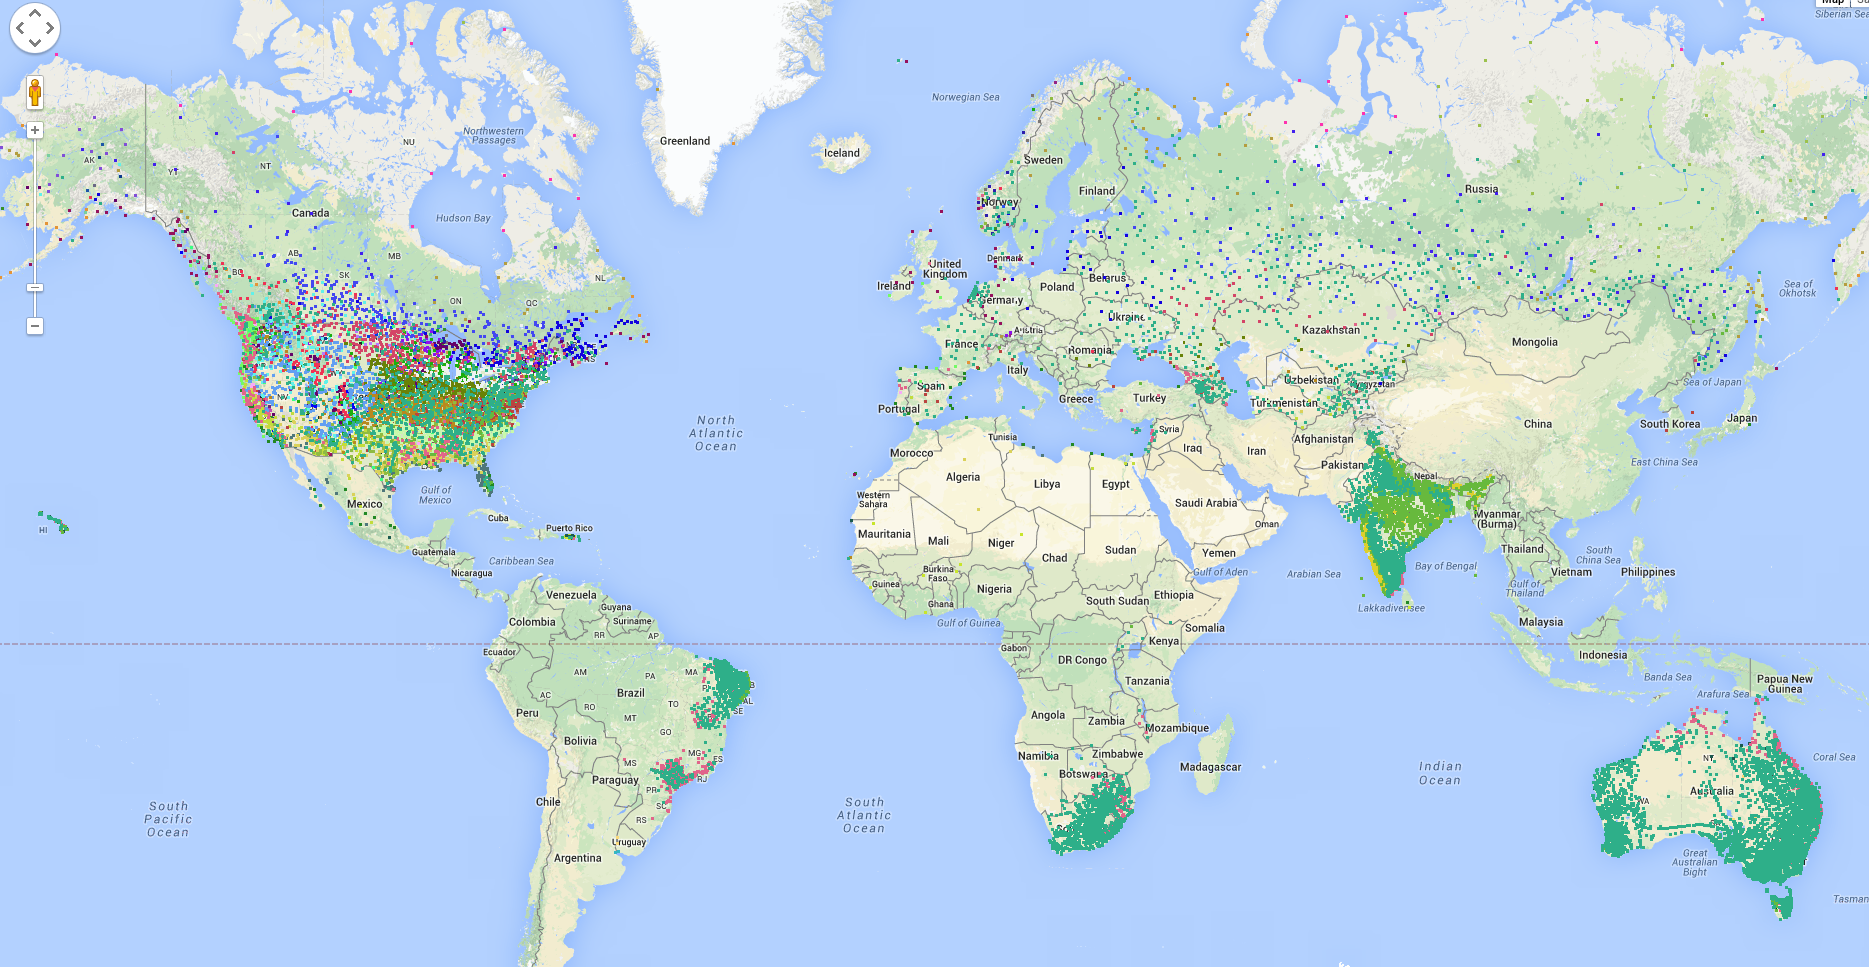
\includegraphics[width =0.8\linewidth]{images/1940.png}\\ 1940\\
        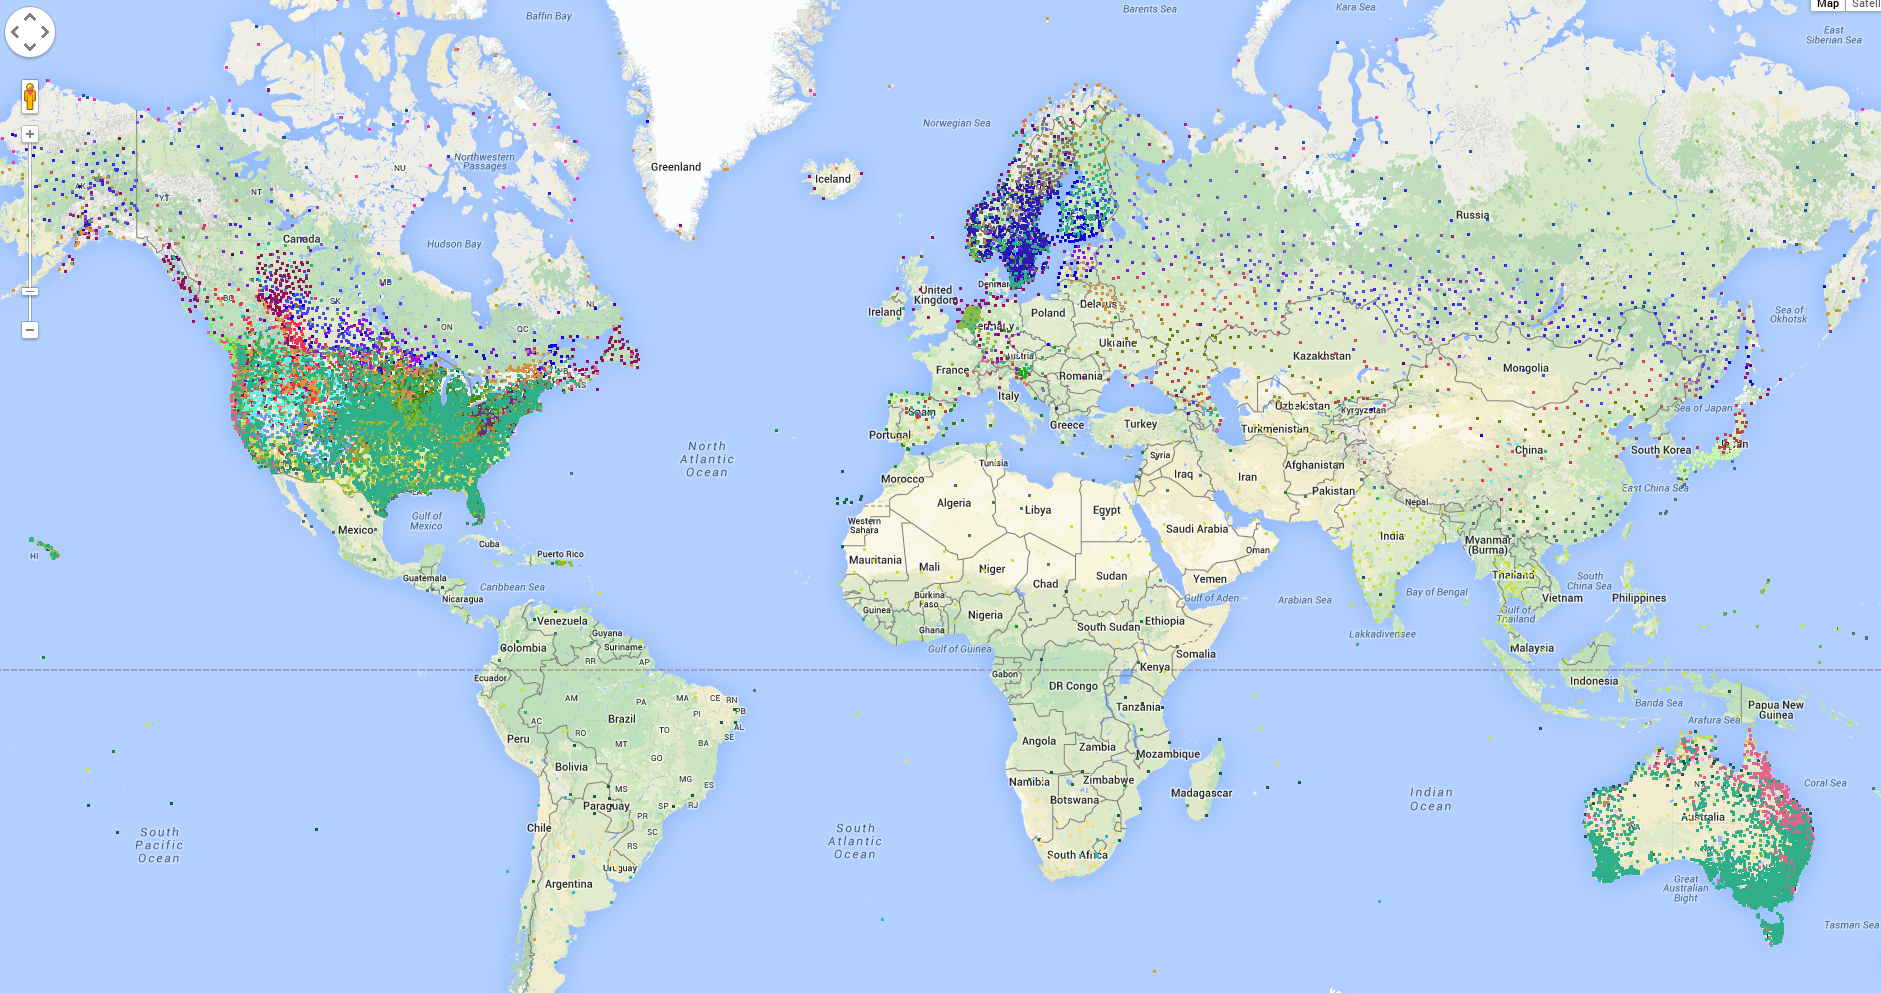
\includegraphics[width =0.8\linewidth]{images/2010.png}\\ 2010\\
    \end{tabular}
    \caption{Clustering results of 1904, 1940 and 2010.}
\end{figure}

Here we observed a similar result as before. 

\subsection{Result of recent $11$ years}

We also extracted the result from $2003$ to $2013$, made a video by Python which is now available on Youtube\cite{youtube}.

\section{Conclusion}

Althgouh the result of our project is quite subjective, there is an optimal number of clusters. After enough iterations, the result remains a good quality. For the ones with less number of clusters, it would take less time to compute while for bigger number of clusters, it would take more time. From \cite{sklearn}'s website, there is a note as following
\begin{quote}
The k-means problem is solved using Lloyd’s algorithm.

The average complexity is given by $O(k n T)$, were n is the number of samples and T is the number of iteration.

The worst case complexity is given by $O(n^{(k+2/p)})$ with n = n\_samples, p = n\_features. (D. Arthur and S. Vassilvitskii, `How slow is the k-means method?' SoCG2006)

In practice, the k-means algorithm is very fast (one of the fastest clustering algorithms available), but it falls in local minima. That’s why it can be useful to restart it several times.
\end{quote}

From Section {\color{red}Introduction}, we can see that the size of data varies a lot. The more data we use, the more time it would take to run. 

\subsection{Difficulties}
\begin{itemize}
    \item The size of Dataset is too big to fit in the memory.
    \item Too inefficient to run K-means on the whole dataset
    \item Install Python tools in the remote machine
\end{itemize}

\subsection{Lecture Learned}
\begin{itemize}
    \item Debug thoroughly before implementing it in a distributed system
    \item Saved the log whenever necessary
\end{itemize}

\section{Future Work}
\begin{itemize}
    \item Create more features and do feature selection
    \item Other clustering algorithm, maybe GMM 
\end{itemize}



%\bibliographystyle{plain}
%\bibliography{Proposal}
\begin{thebibliography}{1}
    \bibitem{EMR} http://aws.amazon.com/elasticmapreduce/
    \bibitem{GHCN-D} Peterson, Thomas C., and Russell S. Vose. ``An overview of the Global Historical Climatology Network temperature database.'' Bulletin of the American Meteorological Society 78.12 (1997): 2837-2849.
    \bibitem{boto} https://boto.readthedocs.org/en/latest/
    \bibitem{S3} http://aws.amazon.com/de/s3/
    \bibitem{sklearn} http://scikit-learn.org/stable/
    \bibitem{GoogleMap} https://developers.google.com/maps/?hl=de
    \bibitem{youtube} https://www.youtube.com/watch?v=xQfEk978IE4\&list=UUkzQg0KkXhibidSnmizd4Vg\&index=2
    \bibitem{world} http://www.ngdc.noaa.gov/mgg/image/color\_etopo1\_ice\_low.jpg
\end{thebibliography}

\end{document}
=======
\documentclass[a4paper]{article}

\usepackage{geometry}
\usepackage{indentfirst}
\usepackage{verbatim}
\usepackage{amsmath,amssymb}
\usepackage{amsthm}
\DeclareMathOperator*{\argmax}{arg\,max}
\usepackage{amsthm}
\usepackage{bm}
\usepackage{bbm}
\usepackage{graphicx}
\usepackage{float}
\usepackage{color}
\usepackage{algorithm}
\usepackage{algorithmic}
%\renewcommand{\algorithmicrequire}{\textbf{Initialization:}}
%\renewcommand{\algorithmicensure}{\textbf{Inference:}}

\geometry{left=3cm,right=3cm,top=3.75cm,bottom=3.75cm}
\setlength{\parindent}{0em}
\setlength{\parskip}{1em}


\begin{document}

\newtheorem{thm}{Theorem}
\newtheorem*{thm*}{Theorem}
\newtheorem{lem}{Lemma}
\newtheorem{cla}{Claim}
\newtheorem{prop}{Proposition}

\title{Final report}

\author{Lei Zhong, Hantian Zhang, Jian Zhang}
\date{}
\maketitle

\abstract{We did more experiment with different parameters during the Milestone 4, optimized the code and visualized the results as a video on youtube\cite{youtube}. In this final report, we will summarize over the whole three-month project, demonstrate the results and point out some future work.}

\section{Introduction}
Climate change is an issue of ever increasing significance to both policy makers and the public, especially as the impact of climate change on global and local economies has become clear. People care about this critical issue, and this interest is reflected in news headlines and across global social media.

Geologists and climatologists have developed many traditional methods the get more insight of this problem. They look into evidences from temperature measurements and proxies, historical and archaeological evidence, glaciers, arctic sea ice loss, vegetation, precipitation, sea level change and so on. They have also built many satellites and monitoring stations that are collecting large volumes of data everyday to help with the analysis. However, these traditional methods are mostly based on hypothesis testing methods and can't make full use of these automatically collected data, as the data volume is too big to handle. It is natural that novel methods that are able to deal with big data can play an important role in the climate change research.

We developed a system to cluster and visualize the GHCN-D data\cite{GHCN-D}.
GHCN-D is a dataset that contains daily weather observations over global land areas.
Like its monthly counterpart, GHCN-Daily is a composite of climate records from
numerous sources that were merged together and subjected to a common suite of quality assurance reviews. The archive includes the following meteorological elements: daily maximum temperature, daily minimum temperature, temperature at the time of observation, precipitation (i.e., rain, melted snow), snowfall, snow depth, other elements where available. The data we used dates from 1763 to 2014 and has approximately 100 Gigabytes total volume.


%Why is this problem interesting or useful?
%Why do we need a new system?
%Which alternative/traditional techniques can be used to solve the problem

%What is the main new contribution of your approach
%How does your solution compare to existing work



\section{Contribution}
\textbf{TO\_DO:}
todo contribution
todo compare to existing work, find some work 



\paragraph{to add}
In addition to coreset sampling, we could also run on the whole feature, 

\section{Performance Measurements and Results}

\subsection{Performance metrics}
There are three common performance metrics, we have our own way to measure:
\begin{itemize}
    \item Execution time: one is run-time, the other is normalized instance hour;
    \item Memory-consumption \& number of machines: peak memory of mapper and reducer, see Table \ref{table:m3}. We use m3.2xlarge and one master, two cores.
    \item Solution quality: our project is quite innovative and there is no existing work. We can only compare our results with differnt parameters by topographical world map\cite{world}.
\end{itemize}

\begin{table}[htbp]
    \centering
    \label{table:m3}
    \begin{tabular}{|l|l|l|l|}
        \hline
        Model & vCPU & Mem (GiB) & SSD Storage (GB) \\
        \hline
        m3.medium & 1 & 3.75 & 1 x 4  \\
        m3.large  & 2 & 7.5 & 1 x 32 \\
        m3.xlarge & 4 & 15 & 2 x 40 \\
        m3.2xlarge& 8 & 30 & 2 x 80 \\
        \hline
    \end{tabular}
    \caption{Instance types}
\end{table}

\subsection{Result of recent four decades}
Same as Milestone $3$, we selected the year $1983$, $1993$, $2003$ and $2013$ to show the results. The size of raw compressed dataset is as showing in the Table \ref{table:4year}.

\begin{table}[htbp]
    \centering
    \label{table:4year}
    \begin{tabular}{|l|l|l|l|l|}
        \hline
        Year & 1983 & 1993 & 2003 & 2013 \\
        \hline
        Compressed Size & 155MB & 152MB & 159MB & 166MB \\
        \hline
        Original & 912.4MB & 899.7MB & 960.7MB & 987.2MB \\
        \hline
    \end{tabular}
    \caption{Size of dataset in selected years}
\end{table}

We kept adjusting the parameters until we found the result is resonable. The following pictures are snapshots from $150$ clusters, $500$ iterations. From the pictures we can see that there do exist some pattern in the same region in different years. But generally, the shape of clusters would note be the same.

\begin{figure}[htbp]
    \centering
    \begin{tabular}{c}
        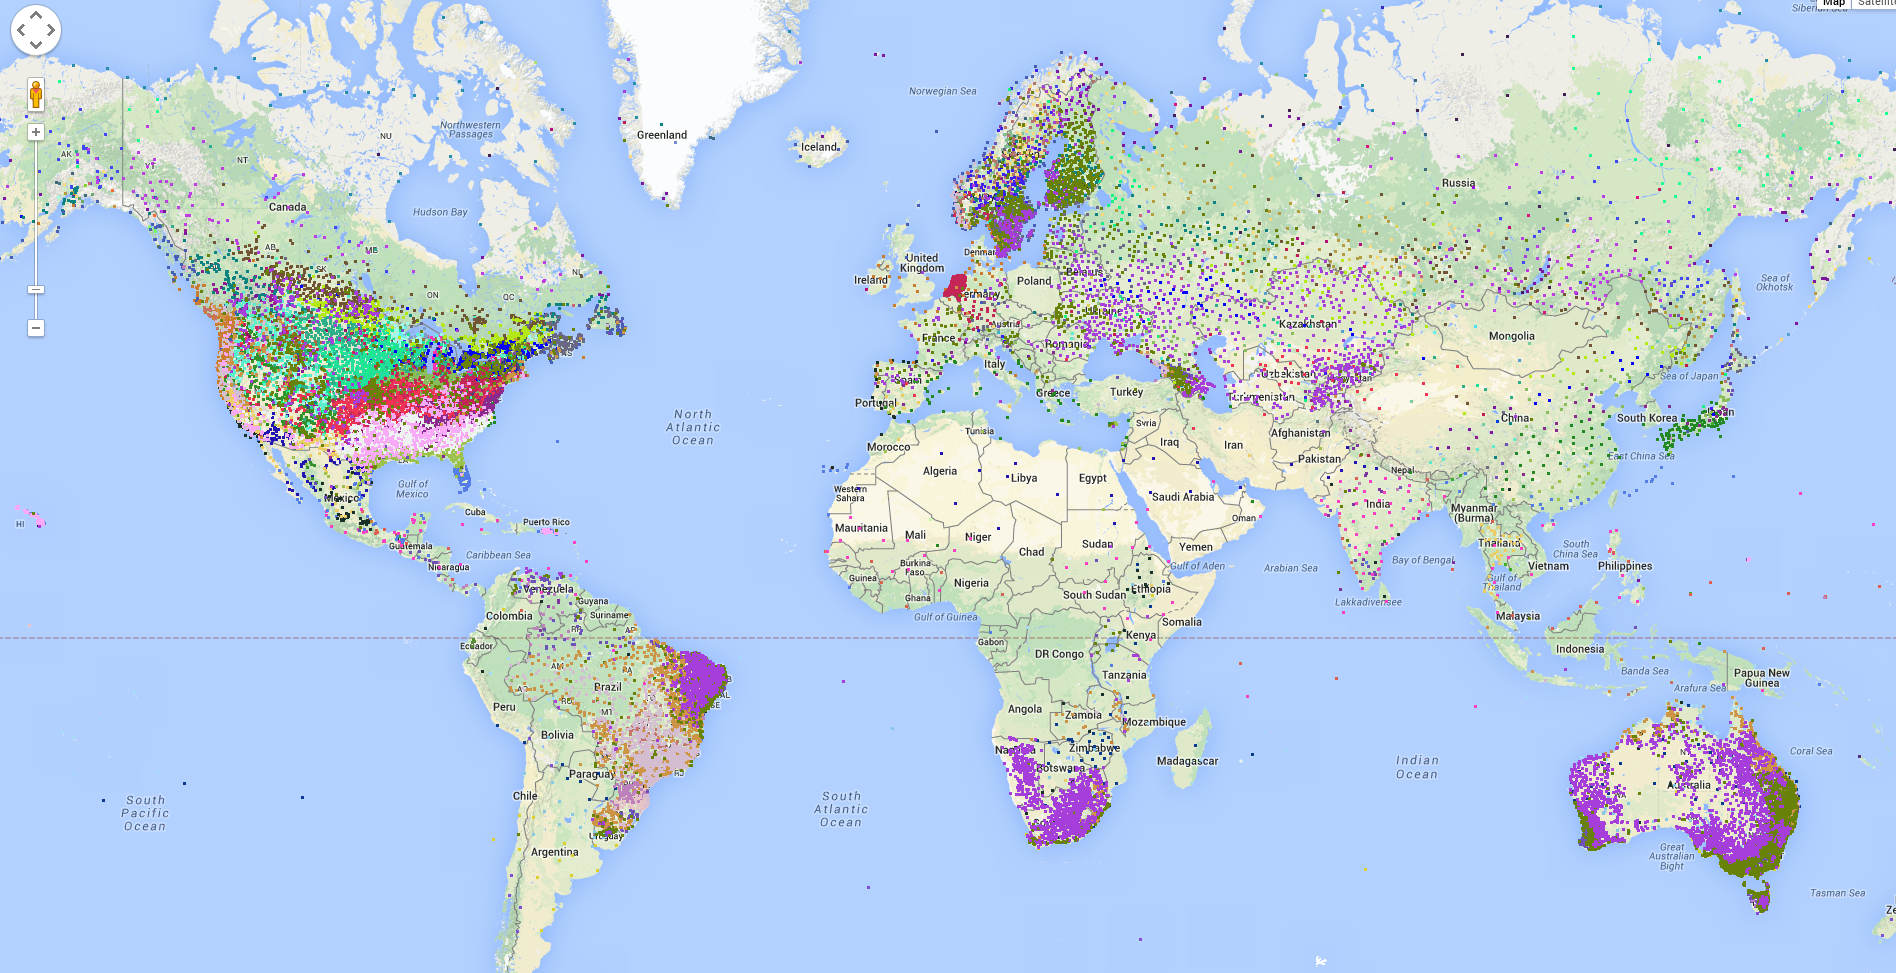
\includegraphics[width =\linewidth]{images/1983.png}\\1983\\
        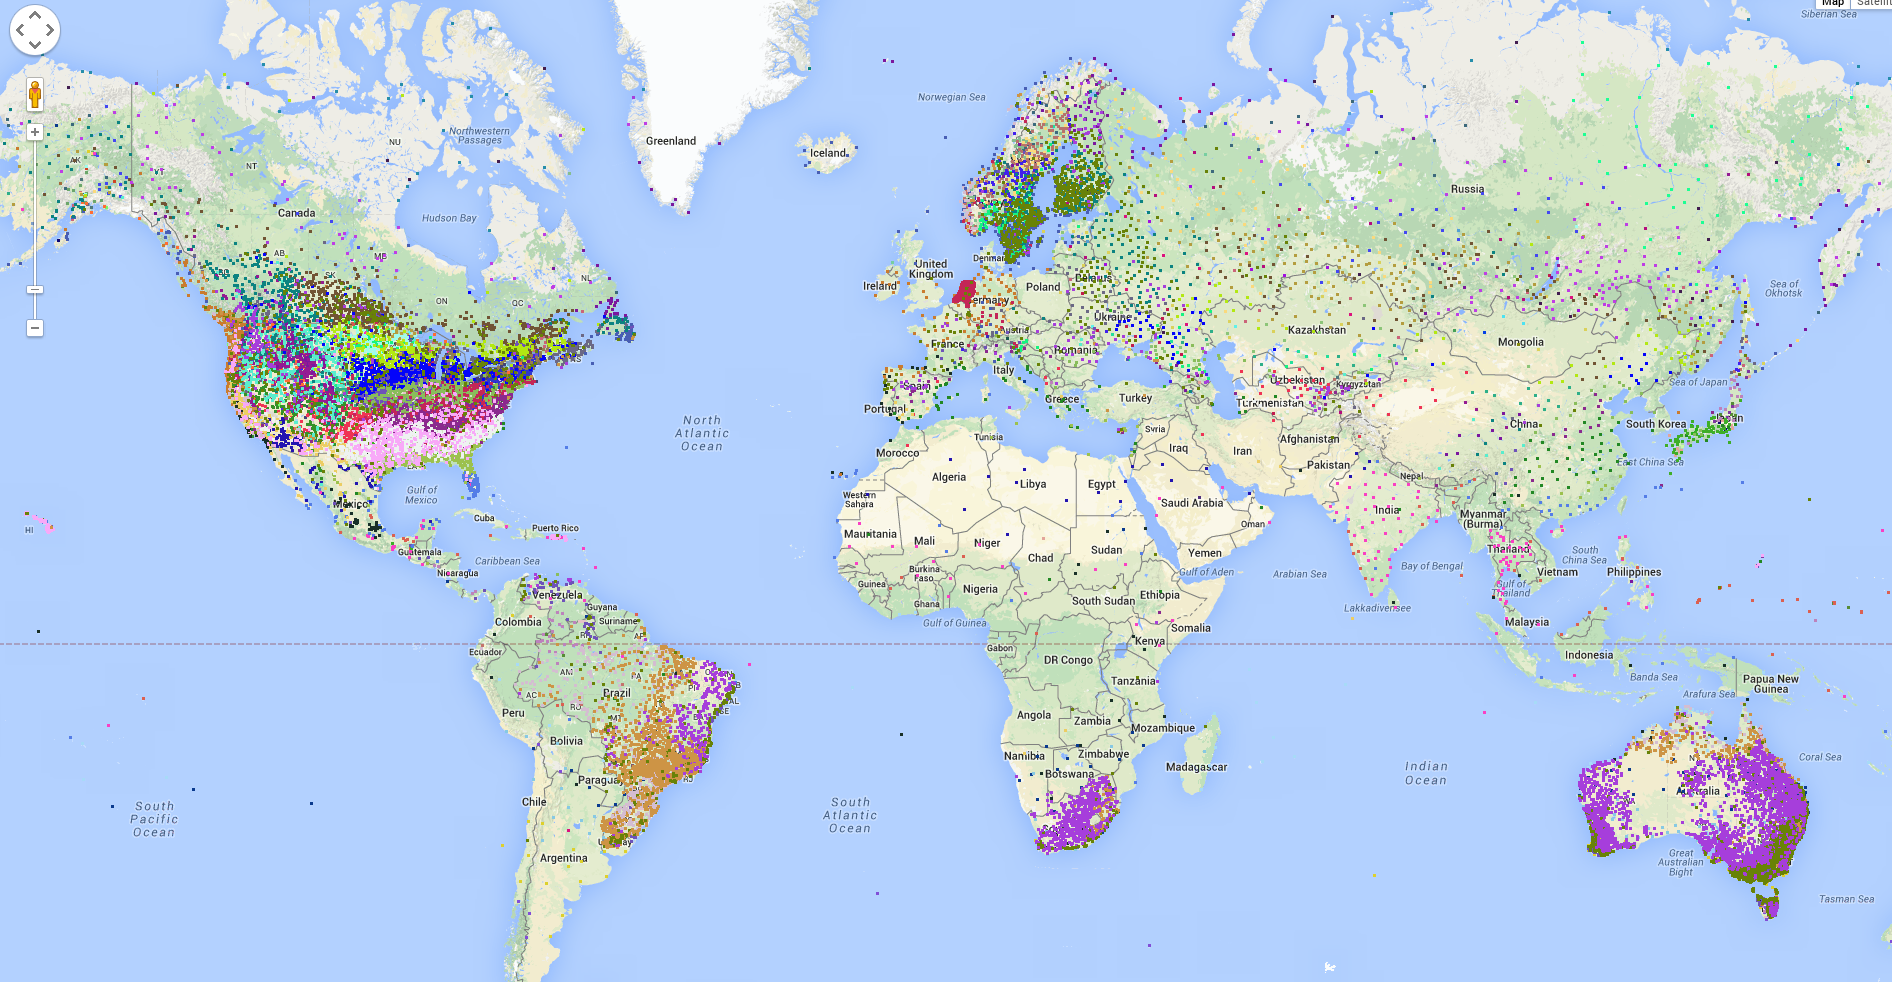
\includegraphics[width =\linewidth]{images/1993.png}\\1993\\
    \end{tabular}
    \caption{Clustering results of 1983 and 1993.}
\end{figure}

\begin{figure}[htbp]
    \begin{tabular}{c}
        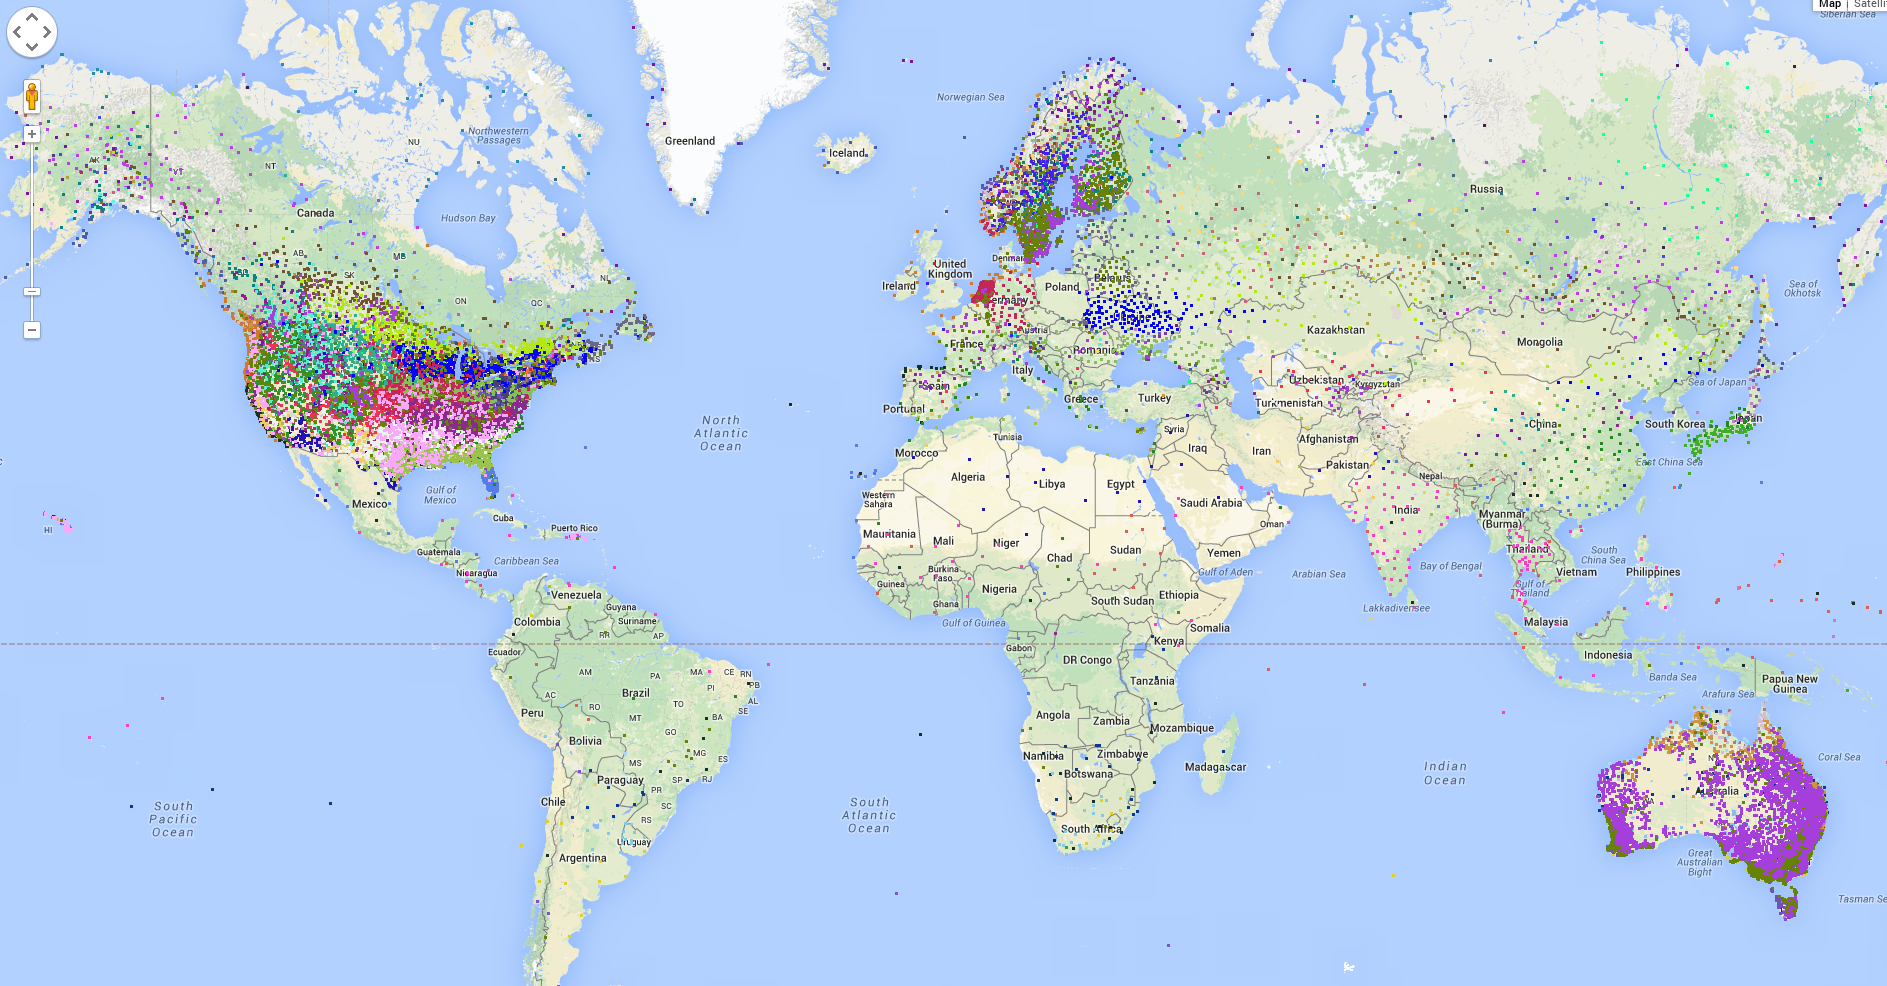
\includegraphics[width =\linewidth]{images/2003.png}\\2003\\
        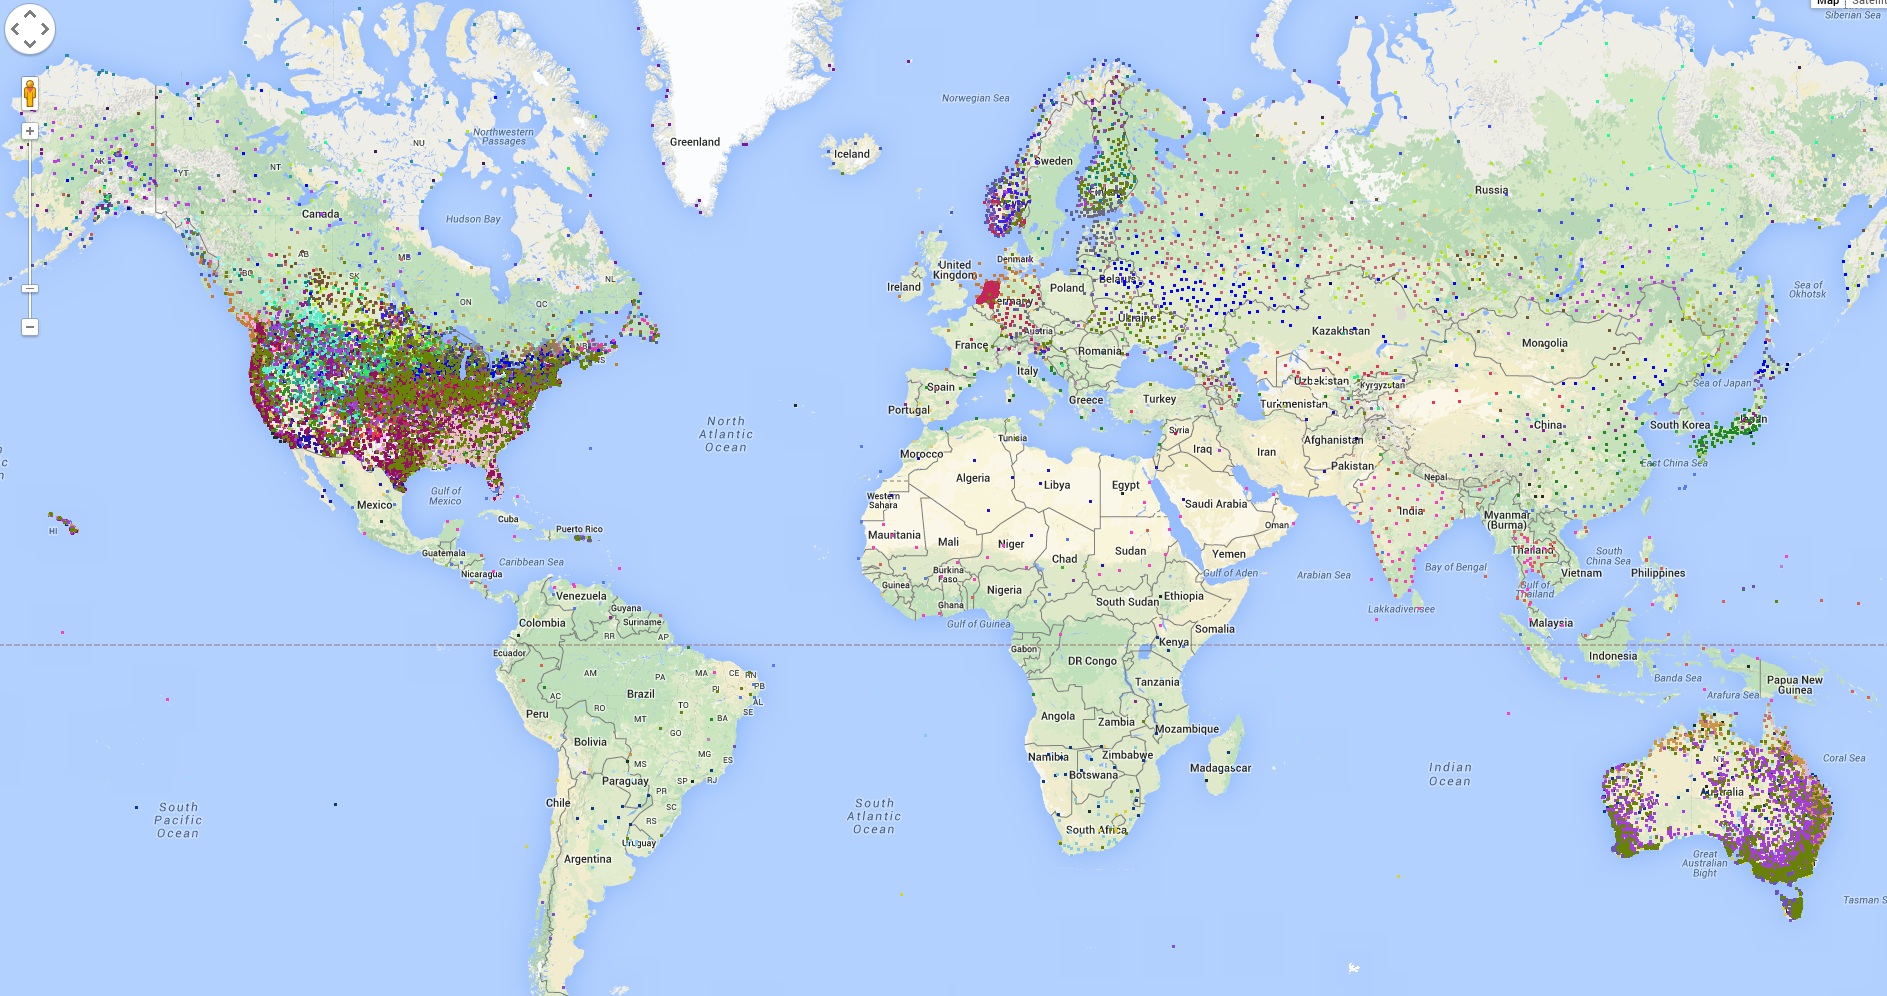
\includegraphics[width =\linewidth]{images/2013.png}\\2013\\
    \end{tabular}
    \caption{Clustering results of 2003 and 2013.}
\end{figure}

Compared with results in milestone $3$, there are two major improvements.
\begin{itemize}
    \item More clusters (which are different colors) are observed;
    \item Less mising points on the map;
\end{itemize}

\subsection{Result of more than a century}

At next step, we adjusted the parameter to less clusters. Because the former years have really small recorded weawther information, it's unnecessary to run many clusters. When we run with $90$ clusters, $500$ iterations to check if there is any similar pattern to the extent of a century. We have chosen the years $1876$, $1896$, $1904$, $1940$, and $2010$ with the size shown in Table \ref{table:5years}. The values are varying from $900K$ to $184M$\footnote{
The results before $1876$ is meaningless since there were not enough data.}.

\begin{table}[htbp]
    \centering
    \label{table:5years}
    \begin{tabular}{|l|l|l|l|l|l|}
        \hline
        Year & 1876 & 1896 & 1904 & 1940 & 2010 \\
        \hline
        Compressed & 900KB & 18MB & 32MB & 73MB & 184MB \\
        \hline
        Original & 5.5MB & 110.2MB & 201.7MB & 441.4MB & 1GB \\
        \hline
    \end{tabular}
    \caption{Size of dataset in selected years}
\end{table}

\begin{figure}[htbp]
    \centering
    \begin{tabular}{c}
        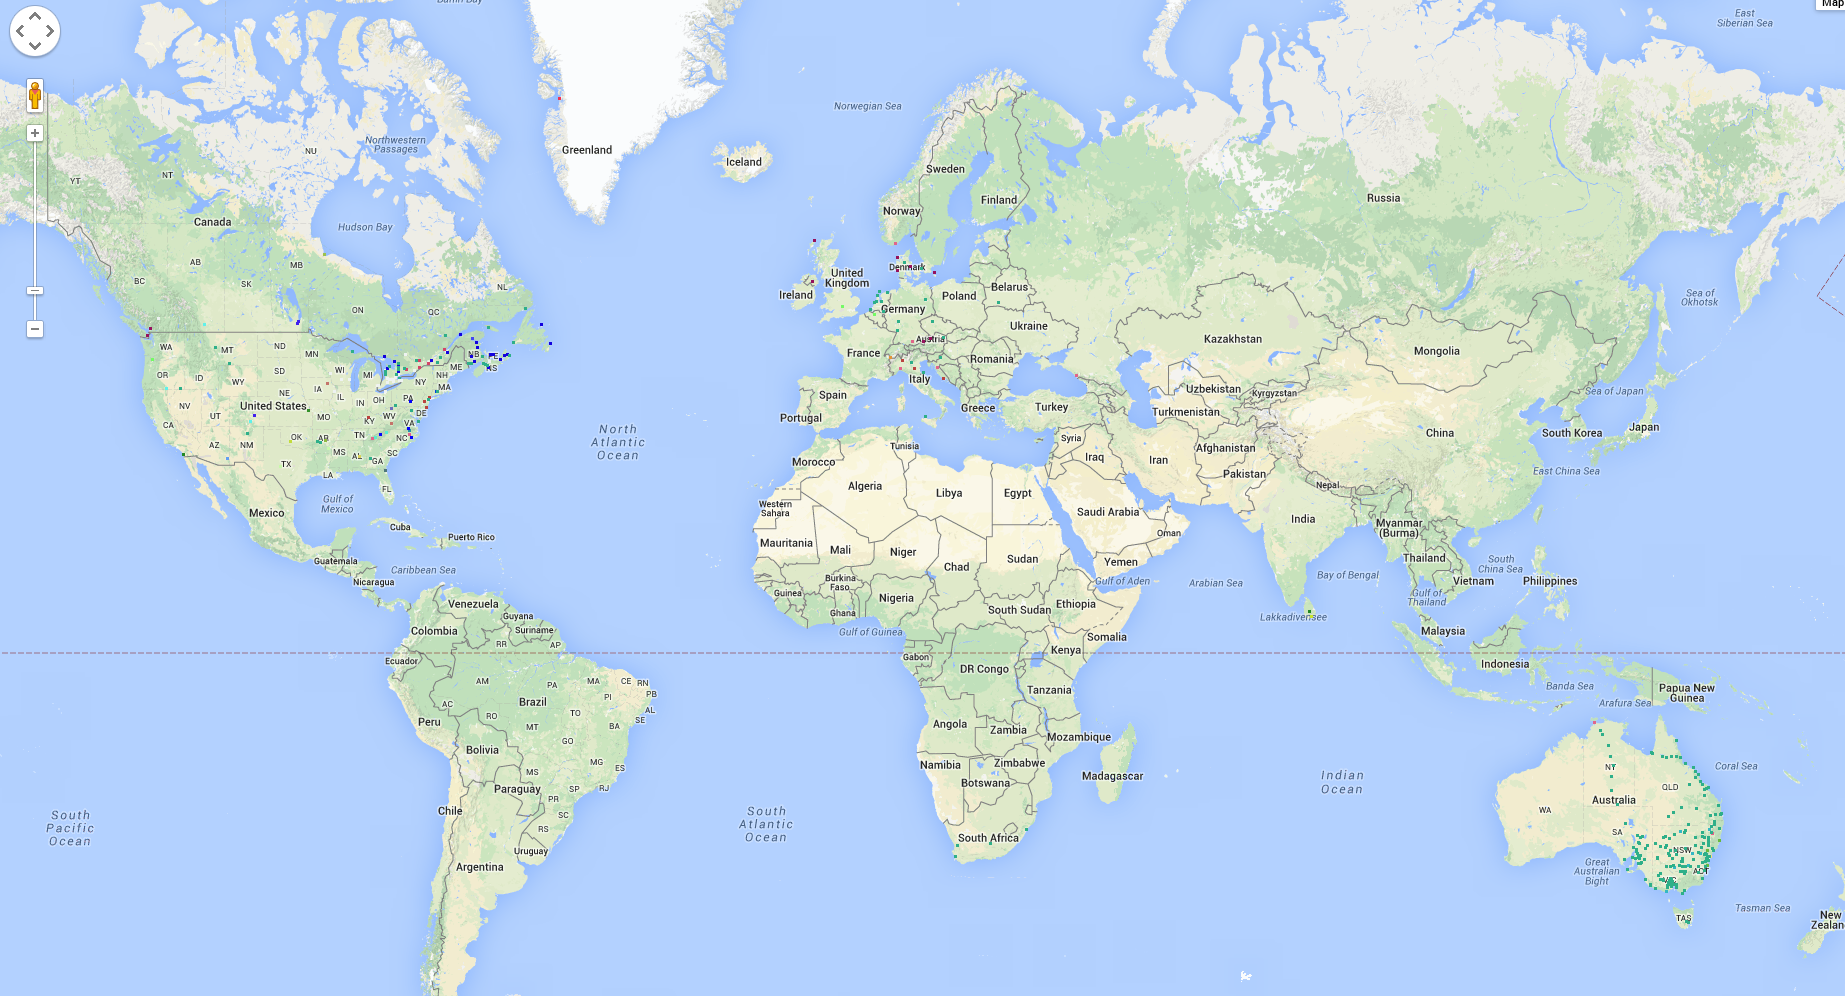
\includegraphics[width =\linewidth]{images/1876.png}\\ 1876\\
        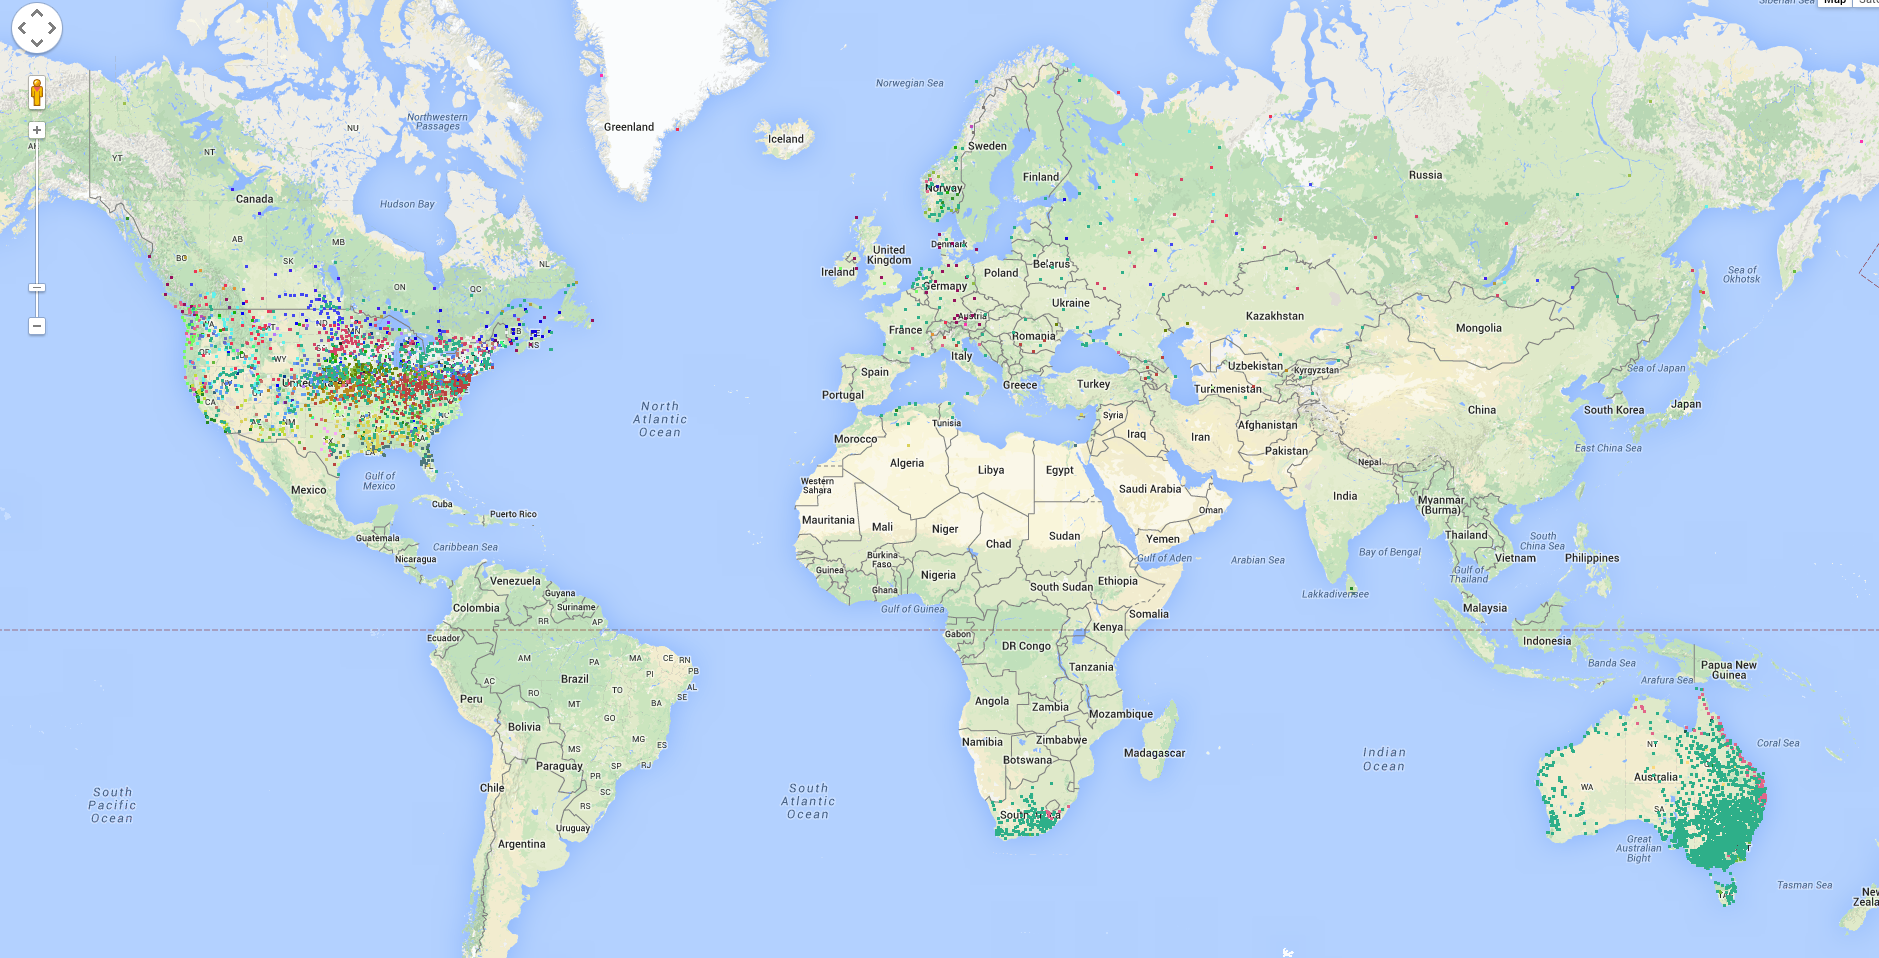
\includegraphics[width =\linewidth]{images/1896.png}\\ 1896\\
   \end{tabular}
    \caption{Clustering results of 1876 and 1896.}
\end{figure}

\begin{figure}[htbp]
    \centering
    \begin{tabular}{c}
        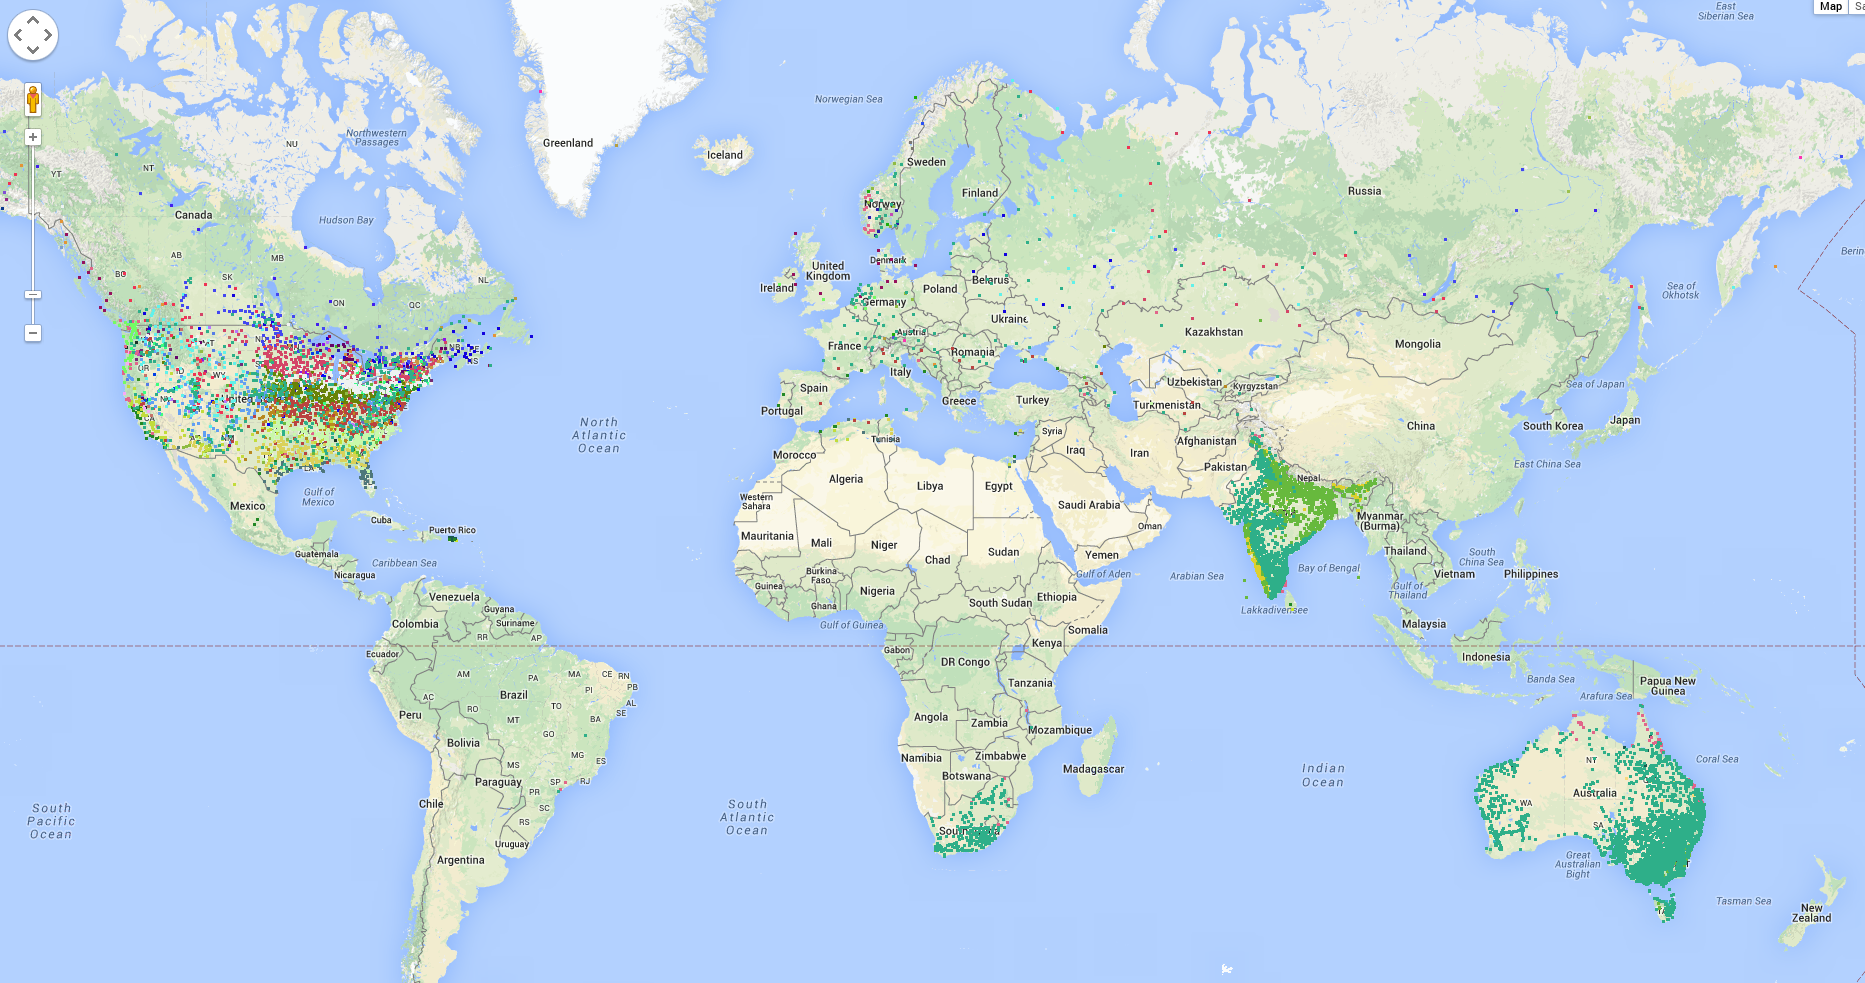
\includegraphics[width =0.8\linewidth]{images/1904.png}\\ 1904\\
        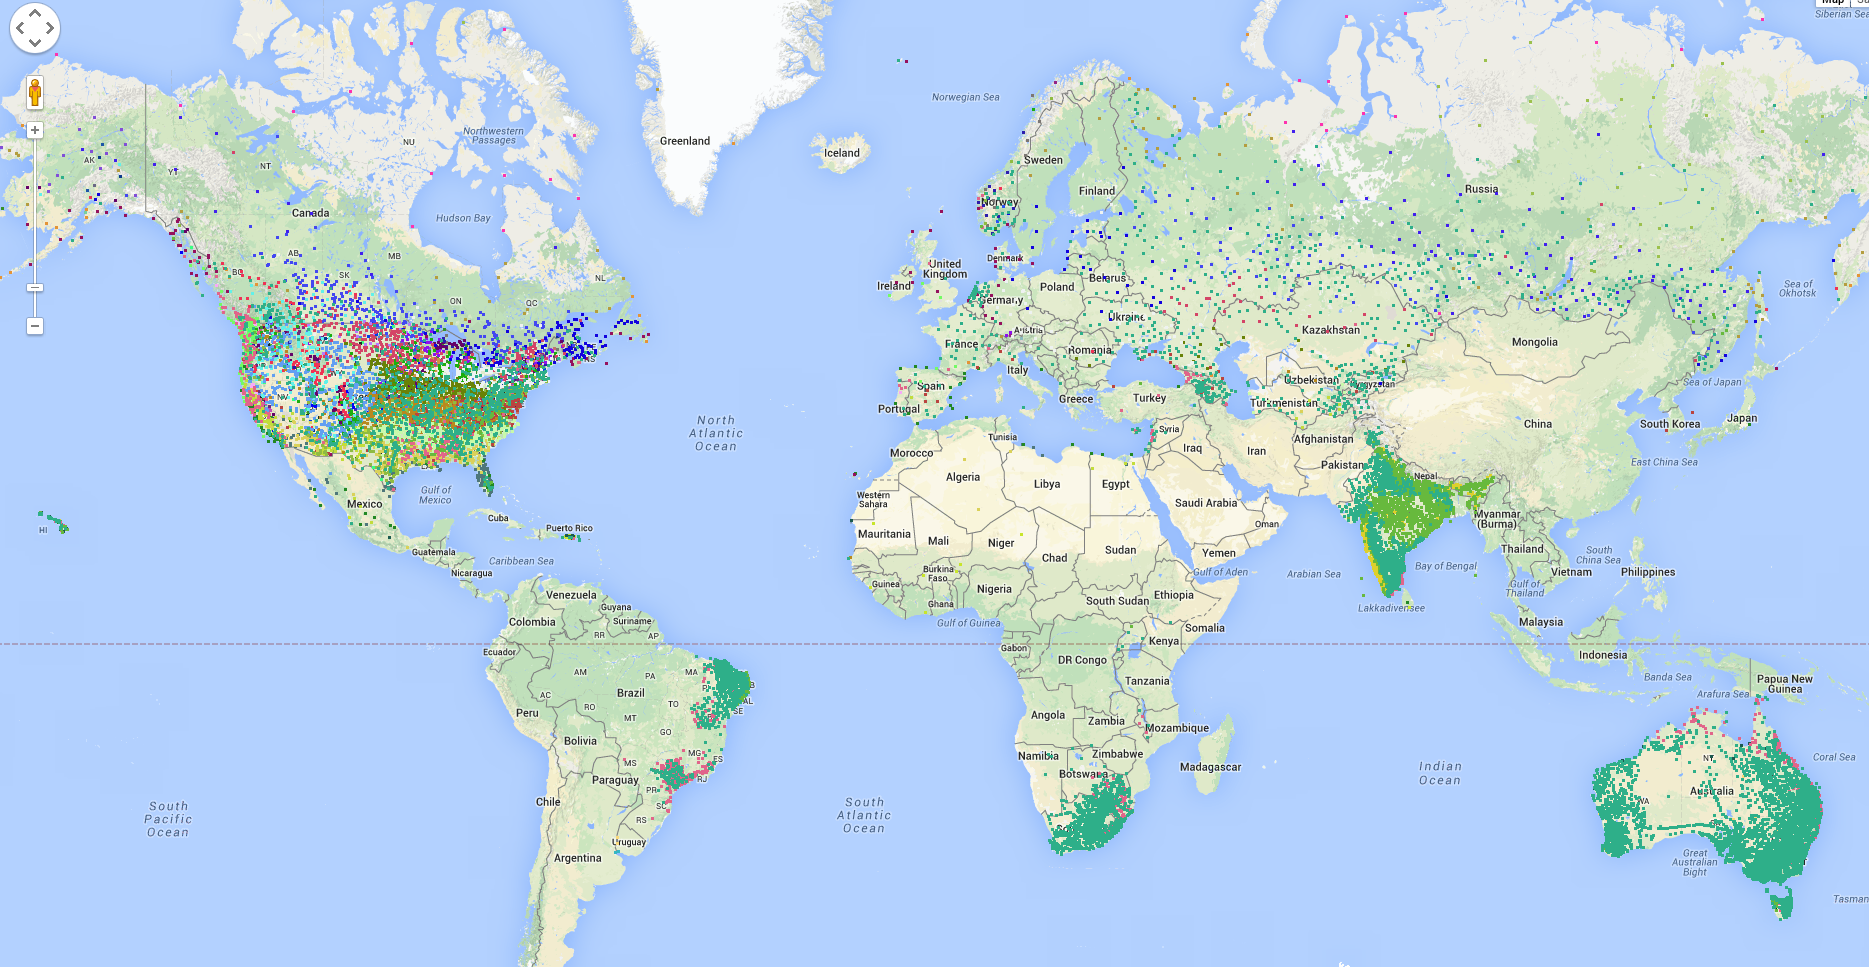
\includegraphics[width =0.8\linewidth]{images/1940.png}\\ 1940\\
        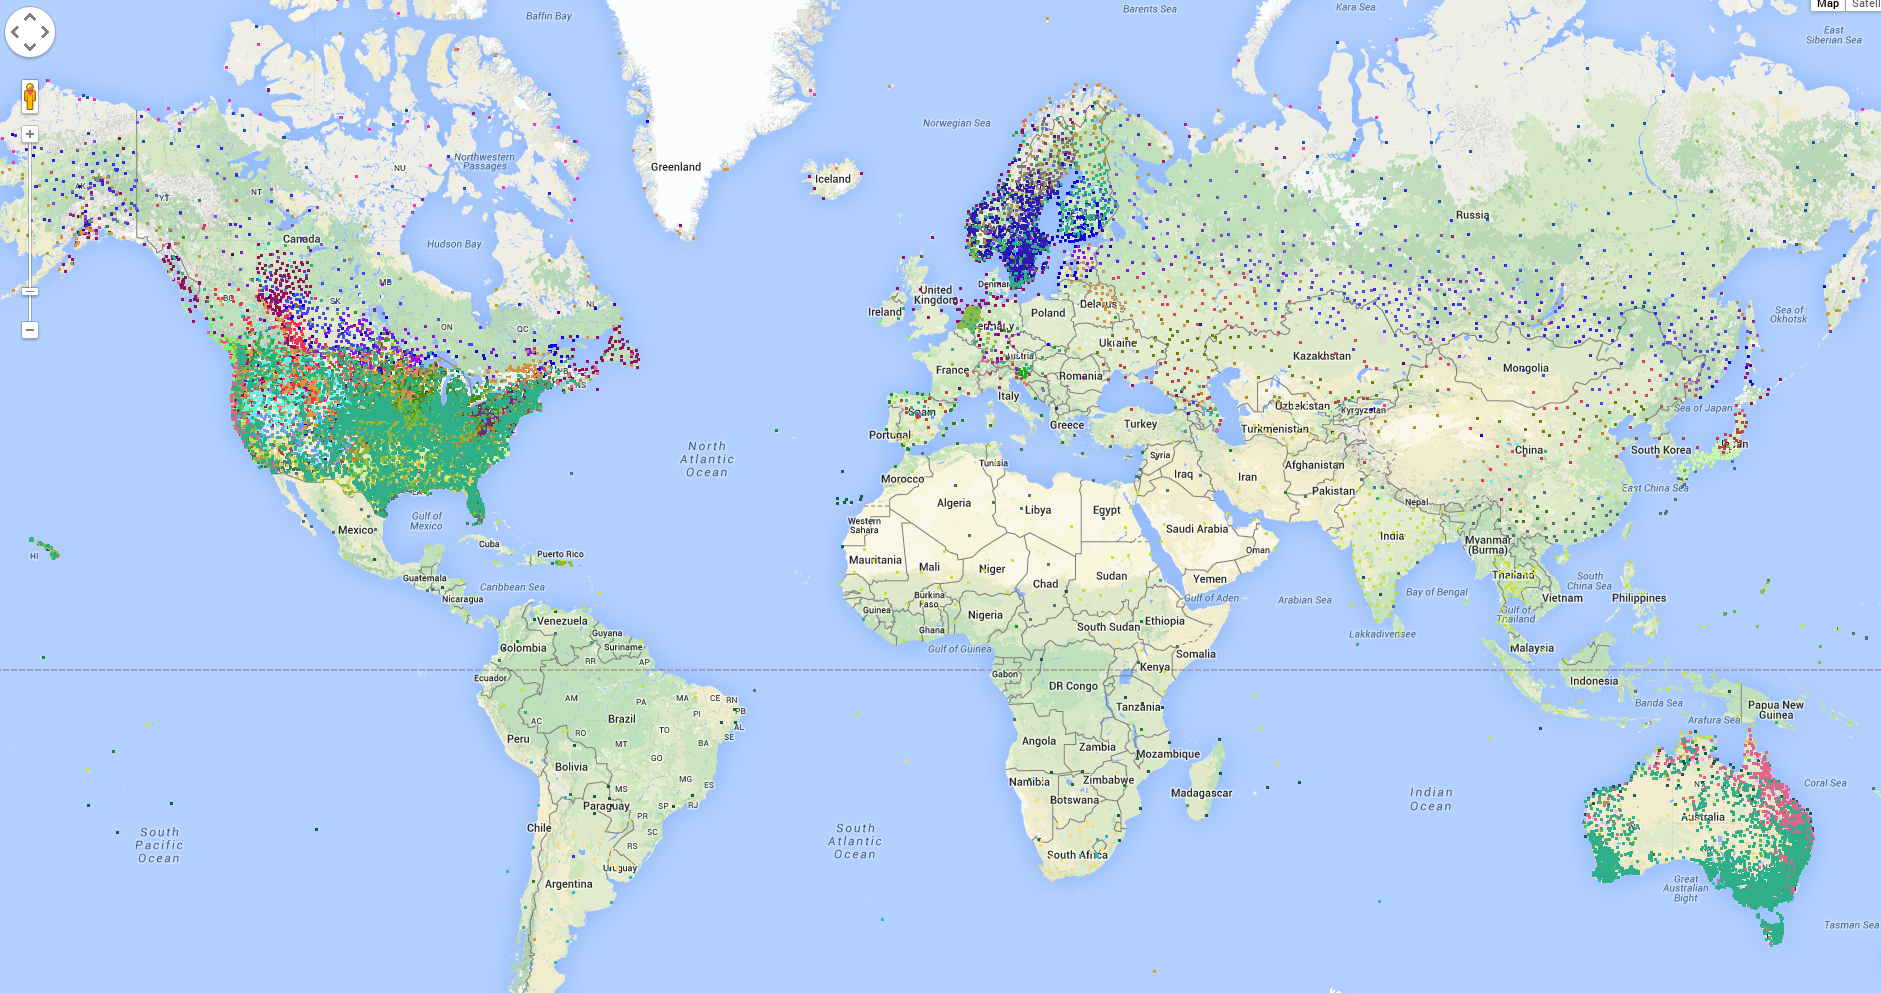
\includegraphics[width =0.8\linewidth]{images/2010.png}\\ 2010\\
    \end{tabular}
    \caption{Clustering results of 1904, 1940 and 2010.}
\end{figure}

Here we observed a similar result as before. 

\subsection{Result of recent $11$ years}

We also extracted the result from $2003$ to $2013$, made a video by Python which is now available on Youtube\cite{youtube}.

\section{Conclusion}

Althgouh the result of our project is quite subjective, there is an optimal number of clusters. After enough iterations, the result remains a good quality. For the ones with less number of clusters, it would take less time to compute while for bigger number of clusters, it would take more time. From \cite{sklearn}'s website, there is a note as following
\begin{quote}
The k-means problem is solved using Lloyd’s algorithm.

The average complexity is given by $O(k n T)$, were n is the number of samples and T is the number of iteration.

The worst case complexity is given by $O(n^{(k+2/p)})$ with n = n\_samples, p = n\_features. (D. Arthur and S. Vassilvitskii, `How slow is the k-means method?' SoCG2006)

In practice, the k-means algorithm is very fast (one of the fastest clustering algorithms available), but it falls in local minima. That’s why it can be useful to restart it several times.
\end{quote}

From Section {\color{red}Introduction}, we can see that the size of data varies a lot. The more data we use, the more time it would take to run. 

\subsection{Difficulties}
\begin{itemize}
    \item The size of Dataset is too big to fit in the memory.
    \item Too inefficient to run K-means on the whole dataset
    \item Install Python tools in the remote machine
\end{itemize}

\subsection{Lecture Learned}
\begin{itemize}
    \item Debug thoroughly before implementing it in a distributed system
    \item Saved the log whenever necessary
\end{itemize}

\section{Future Work}
\begin{itemize}
    \item Create more features and do feature selection
    \item Other clustering algorithm, maybe GMM 
\end{itemize}



%\bibliographystyle{plain}
%\bibliography{Proposal}
\begin{thebibliography}{1}
    \bibitem{EMR} http://aws.amazon.com/elasticmapreduce/
    \bibitem{GHCN-D} Peterson, Thomas C., and Russell S. Vose. ``An overview of the Global Historical Climatology Network temperature database.'' Bulletin of the American Meteorological Society 78.12 (1997): 2837-2849.
    \bibitem{boto} https://boto.readthedocs.org/en/latest/
    \bibitem{S3} http://aws.amazon.com/de/s3/
    \bibitem{sklearn} http://scikit-learn.org/stable/
    \bibitem{GoogleMap} https://developers.google.com/maps/?hl=de
    \bibitem{youtube} https://www.youtube.com/watch?v=xQfEk978IE4\&list=UUkzQg0KkXhibidSnmizd4Vg\&index=2
    \bibitem{world} http://www.ngdc.noaa.gov/mgg/image/color\_etopo1\_ice\_low.jpg
\end{thebibliography}

\end{document}